\documentclass[12pt]{article}
\usepackage[left=3.5cm,right=2cm,top=2.5cm,bottom=2.5cm]{geometry}
\usepackage[T1]{fontenc}
\usepackage[utf8]{inputenc}
\usepackage{tgpagella}
\usepackage{enumerate}
\usepackage{url}
\usepackage{multirow}
\usepackage{longtable}
\usepackage{polski}
\usepackage{graphicx}
\usepackage{float}
\usepackage{color}
\usepackage{amsmath}
\usepackage{longtable}
\usepackage{tabularx}
\usepackage{ltablex,booktabs}
\usepackage{amssymb}
\usepackage{rotating}
\usepackage{subfigure}
\usepackage{float}
\usepackage{tabu}
\usepackage{caption}
\usepackage{footnote}
\usepackage{xspace}
\usepackage{mathpazo}
\usepackage[table]{xcolor}
\usepackage[justification=centering]{caption}
\graphicspath{ {images/} }

\pagestyle{empty}

\title{\LARGE{Uniwersytet Wrocławski}\\
\Large{Wydział Matematyki i Informatyki}\\
\large{Kierunek: Informatyka}}

\date{}

\begin{document}
\pagestyle{empty}

\begin{titlepage}
\maketitle
\thispagestyle{empty}


\begin{center}
\author{\LARGE{Adrian Mularczyk}}
\vspace{30pt}

\huge{\textbf{Stworzenie wydajnego wzorca wstrzykiwania zależności dla złożonych grafów zależności}}
\vspace{50pt}
\end{center}

\begin{flushright}
\large{Praca wykonana pod kierunkiem}
\large{dr. Wiktora Zychli}
\end{flushright}

\vfill
\begin{center}
\begin{large}
Wrocław, 2016
\end{large}
\end{center}
\end{titlepage}

\setlength{\parindent}{0pt}	%usunięcie wcięć
\setlength{\parskip}{1.5ex} 
\renewcommand*{\figurename}{Rys.}
\renewcommand*{\tablename}{Tab.} 
\renewcommand{\captionsize}{\small}

\setlength{\intextsep}{0pt}

\clearpage

\tableofcontents



\clearpage
\begin{center}
\textbf{Streszczenie}\\
\vspace{16pt}
\textbf{Stworzenie wydajnego wzorca wstrzykiwania zależności dla złożonych grafów zależności}
\end{center}
Wstrzykiwanie zależności jest to zbiór zasad projektowania oprogramowania, które umożliwiają luźne powiązania, a dzięki temu kod jest rozszerzalny i łatwiejszy w utrzymaniu. Celem tej pracy było stworzenie takiej realizacji, która będzie sprawdzała się dla złożonych grafów zależności. Aplikacja została napisana w języku C\# z wykorzystaniem przestrzeni nazw Reflecion.Emit oraz jest w pełni przetestowana. W aplikacji zaproponowano dwa rozwiązania, które działają niezależnie i można ich używać naprzemiennie. Testowy wydajnościowe zostały przeprowadzone przy użyciu aplikacji, która powstała na potrzeby tej pracy. Porównano w nich 5 najbardziej popularnych i 4 najszybsze rozwiązania. Końcowe wyniki wykazały, że z obecnie dostępnych rozwiązań na rynku, moje radzi sobie najlepiej.




\clearpage
\section{Wstęp}
\subsection{Cel pracy}
Wstrzykiwanie zależnośc jest wzorcem projektowym, który pozwala na tworzenie kodu o luźniejszych powiązaniach, łatwiejszego w testowaniu i modyfikacji. Najbardziej popularnymi implementacjami tego wzorca w języku C\# są Unity i Ninject. Niestety większość rozwiązań skupia się na zapewnieniu jak największej liczby funkcjonalności, co ma negatywne skutki jeśli chodzi o wydajność. O ile przy małej ilości zależności te czasy nie są zbyt duże, to wraz ze wzrostem zależności wydajność dość mocno daje o sobie znać. Celem niniejszej pracy magisterskiej jest stworzenie takiej implementacji tego wzorca, która będzie wydajna dla złożonych grafów zależności, ale również będzie dostarczać niezbędną funkcjonalności. Do tego celu zostaną wykorzystane mechanizmy z przestrzeni nazw Reflection.Emit. W tej pracy zostaną przedstawione dwa rozwiązania tego problemu.

\subsection{Układ pracy}
Poza wstępem i podsumowaniem praca składa się jeszcze z czterech rozdziałów. Pierwszy z nich opisuje idee idące za wstrzykiwaniem zależności. W kolejnym znajduje się opis teoretyczny czym jest wstrzykiwanie zależności. Następny rozdział został poświęcony moje implementacji tego wzorca. Ostatni z tych czterech rozdziałów skupia się na testach wydajnościowych, w którym porównuję moje rozwiązanie z kilkoma najbardziej popularnym i kilkoma najwydajniejszymi rozwiązaniami.



\clearpage
\section{Odwrócenie zależności}
\subsection{SOLID}
Na przestrzeni lat powstało bardzo dużo projektów. Część z nich była łatwiejsza w utrzymaniu, część trudniejsza. Analizując te projekty ludzie doszli do wniosku, że są pewne zasady, które powodują, że projekty rozwija się łatwiej. Te zasady zostały połączone w zbiory zasad. Najbardziej popularnych i powrzechnie stosowanym zbiorem zasad jest SOLID \cite{SOLID}:
\begin{itemize}
	\item S (Single responsibility principle) - Klasa powinna mieć tylko jedną odpowiedzialność (nigdy nie powinien istnieć więcej niż jeden powód do modyfikacji klasy).
	\item O (Open/closed principle) - Klasy powinny być otwarte na rozszerzenia i zamknięte na modyfikacje.
	\item L (Liskov substitution principle) - Funkcje które używają klas bazowych, muszą być w stanie używać również obiektów klas dziedziczących po klasach bazowych, bez dokładnej znajomości tych obiektów.
	\item I (Interface segregation principle) - Wiele dedykowanych interfejsów jest lepsze niż jeden ogólny.
	\item D (Dependency inversion principle) - Wysokopoziomowe moduły nie powinny zależeć od modułów niskopoziomowych - zależności między nimi powinny wynikać z abstrakcji.
\end{itemize}
Ta praca w dużej mieże skupia się na rozwiązaniu dla zasady D - Dependency inversion principle. 

\subsubsection{Przykład dla zasady D}
Rysynek \ref{fig:Solid_without} przedstawia przykład przed zastosowaniem zasady D.\\
\begin{figure}[H]
	\begin{center}
  		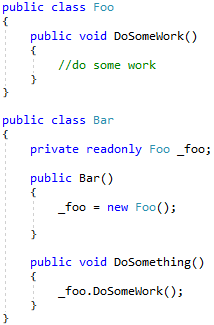
\includegraphics{Solid_without.png}
  		\caption{Przykładowa klasa bez zasady D}
  		\label{fig:Solid_without}
	\end{center}
\end{figure}
Rysunek \ref{fig:Solid_with} przedstawia przykład po zastosowaniu zasady D.\\
\begin{figure}[H]
	\begin{center}
  		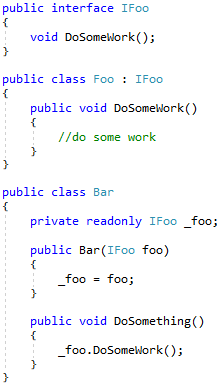
\includegraphics{Solid_with.png}
  		\caption{Przykładowa klasa z zasadą D}
  		\label{fig:Solid_with}
	\end{center}
\end{figure}
Łatwo zauważyć, że teraz klasę Bar nie interesuje implementacja klasy Foo. Jest ona od niej zupełnie niezależna. Spodziewa się jedynie, że dostanie implementację interfejsu IFoo, który dostarcza metodę DoSomeWork. Dzięki takiemu podejściu w łatwy sposób można podmienić implementację interfejsu IFoo w klasie Bar. Zatem tworząc ciało metody DoSomething w klasie Bar nie przejmujemy się implementacją metody DoSomeWork, tylko skupiamy się na tym co metoda DoSomething ma faktycznie robić.
Kolejną zaletą takiego podejścia jest to, że teraz łatwy sposób można przetesować metodę DoSomething - można stworzyć przykładową implementację interfejsu IFoo lub użyć mock'a (zewnętrznej biblioteki, która stworzy pozorną implementację interfejsu za nas). Wcześniej ta metoda nie mogła zostać przetestować przed ukończeniem metody DoSomeWork.


\subsection{Kontenery wstrzykiwania zależności}
Aby można było z powodzeniem stosować zasadę D, należy mieć miejsce gdzie możnaby zdefiniować jakiej klasy obiekt należy podstawić w miejsce interfejsu. Do tego celu używa się kontenerów wstrzykiwania zależności.\\
Kontenery dostarczają nam kilku funkcjonalności. Jedną z nich jest oczywiście możliwość zdefiniowania obiekt jakiej klasy należy zwrócić w miejsce konkretnego interfejsu, ale również umożliwiają stworzenie instancji obiektu konkretnej klasy lub interfejsu. Dodatkowo zapewniają sposobność do rozwiązywania zależności, czyli stworzenia obiektów od których danym obiekt zależy. Niektóre kontenery dostarzcają również mechanizmy pozwalające rozszerzyć tworzenie nowych instancji (co sprzyja osiągnięciu efektów programowania aspektowego).



\clearpage
\section{Wstrzykiwanie zależności}
\subsection{Wstęp}
Jest to zbiór zasad projektowania oprogramowania i wzorców, które pozwalają nam rozwijać luźno powiązany kod.\\
Jakiemu celowi ma służyć wstrzykiwanie zależności? Wstrzykiwanie zależnści nie jestem celem samym w sobie, raczej jest to środek do celu. Ostatecznie celem większości technik programowania jest dostarczenie jak najwydajniej działającego oprogramowania. Jednym z aspektów tego jest napisanie utrzymywalnego kodu.\\
O ile nie pisze się prototypu lub aplikacji, które nigdy nie mają kolejnych wersji (kończą się na wersji 1), to wkrótce będzie trzeba zająć się utrzymaniem i rozwijaniem istniejącego kodu. Aby być w stanie pracować wydajnie z takim kodem bazowym, musi on być jak najlepiej utrzymywalny.\\
Wstrzykiwanie zależności jest niczym więcej niż techniką, która umożliwia luźne powiązania, a luźne powiązania sprawiają, że kod jest rozszerzalny i łatwy w utrzymaniu.\cite{dependency_injection}\\
Wstrzykiwanie zależności może odbywać się na 3 sposoby:
\begin{itemize}
	\item wstrzykiwanie przez konstruktor
	\item wstrzykiwanie przez metodę
	\item wstrzykiwanie przez właściwość
\end{itemize}

\subsubsection{Wstrzykiwanie przez konstruktor}
Jest to główny i najbardziej popularny sposób wstrzykiwania zależności. Niektóre klasy mają kilka konstruktor i atrybut "DependencyConstructor" przydaje się wtedy do oznaczenia, który z nich ma zostać wybrany przy tworzeniu nowego obiektu. Jednakże nie zawsze jest on potrzebny. W większości przypadków klasy mają tylko jeden konstruktor, a także rozwiązania przemsysłowe mają logikę, która wybierze odpowiedni konstruktor (np. ten oznaczony atrybutem, albo ten co ma najwięcej parametrów, albo ten co ma najmniej parametrów). Przykład klasy z atrybutem DependencyConstructor przedstawia Rys. \ref{fig:DependencyConstructor}.\\
\begin{figure}[H]
	\begin{center}
  		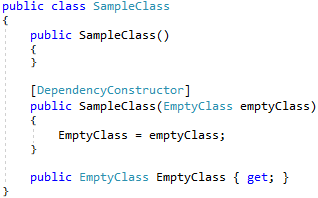
\includegraphics{DependencyConstructor.png}
  		\caption{Przykładowa klasa z atrybutem DependencyConstructor}
  		\label{fig:DependencyConstructor}
	\end{center}
\end{figure}

\subsubsection{Wstrzykiwanie przez metodę}
W przemysłowych rozwiązaniach to wstrzykiwanie z reguły odbywa się albo poprzez oznaczenie metody przez którą chcemy wstrzyknąć zaleźności odpowiednim atrybutem, albo przy rejestracji danej klasy definiujemy przez jakie metody chcemy wstrzyknąć zależności. Przykład klasy z oznaczeniem metody odpowiednim atrybutem przedstawia Rys. \ref{fig:DependencyMethod}.\\
\begin{figure}[H]
	\begin{center}
  		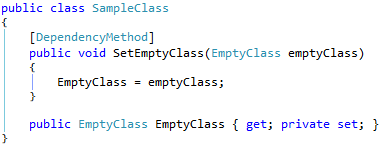
\includegraphics{DependencyMethod.png}
  		\caption{Przykładowa klasa z atrybutem DependencyMethod}
  		\label{fig:DependencyMethod}
	\end{center}
\end{figure}

\subsubsection{Wstrzykiwanie przez właściwość}
Tutaj podobnie jak dla wstrzykiwania przez metodę w przemysłowych rozwiązaniach to wstrzykiwanie z reguły odbywa się albo poprzez oznaczenie właściwoci przez którą chcemy wstrzyknąć zaleźności odpowiednim atrybutem, albo przy rejestracji danej klasy definijumey przez jakie właściwości chcemy wstrzyknąć zależności. Przykład klasy z oznaczeniem właściwości odpowiednim atrybutem przedstawia Rys. \ref{fig:DependencyProperty}.\\
\begin{figure}[H]
	\begin{center}
  		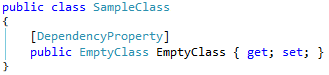
\includegraphics{DependencyProperty.png}
  		\caption{Przykładowa klasa z atrybutem DependencyProperty}
  		\label{fig:DependencyProperty}
	\end{center}
\end{figure}


\subsection{Implementacje przemysłowe}
Na rynku jest wiele implementacji wstrzykiwania zależności. Przedstawię tutaj kilka najbardziej popularnych (według ilości pobrań z NuGet) oraz kilka najszybszych (według rankingu na stronie: http://www.palmmedia.de/Blog/2011/8/30/ioc-container-benchmark-performance-comparison). Dane zostały wzięte z dnia 21-02-2017. W nawiasie znajduje się wersja implementacji, która została użyta w testach (najnowsza na ten dzień).\\
\\
Najbardziej popularne:
\begin{itemize}
	\item Unity (4.0.1) - ponad 5.2 mln pobrań
	\item NInject (3.2.2) - ponad 4.0 mln pobrań
	\item Autofac (4.3.0) - ponad 3.7 mln pobrań
	\item StructureMap (4.4.3) - ponad 1.6 mln pobrań
	\item Windsor (3.4.0) - ponad 1.4 mln pobrań
\end{itemize}
Najszybsze:
\begin{itemize}
	\item Grace (5.1.0)
	\item DryIoc (2.10.1)
	\item LightInject (5.0.1)
	\item SimpleInjector (3.3.2)
\end{itemize}



\clearpage
\section{Implementacja}
Kod źródłowy programu jest dostępnym w repozytorium pod adresem:\\
\url{https://github.com/amularczyk/NiquIoC}\\
Znajduje się tam również kod programu, który posłużył do wykonania testów wydajnościowych, a także ta praca napisana w języku LateX i wszystkie obrazki.

\subsection{Środowisko pracy}
Prac oraz wszystkie testy powstały na komputerze z parametrami:
\begin{itemize}
	\item Intel Core i7-4720HQ (2.60GHz)
	\item 12 GB pamięci RAM
	\item Dysk SSD
\end{itemize}
Narzędzia użyte do stworzenia pracy i testów:
\begin{itemize}
	\item System operacyjny Windows 10 Pro
	\item .Net Framework w wersji 4.6.1
	\item Visual Studio 2017 Comunnity
	\item MSTest
	\item ReSharper
	\item dotCover
	\item Dia
\end{itemize}


\subsection{Wstęp}
Na początku chciałbym pokrótce opisać dwie rzeczy, które są istotne dla mojego rozwiązania. Pierwszą z nich jest Microsoft Intermediate Language, a drugą przestrzeń nazw Reflection.Emit.

\subsubsection{Microsoft Intermediate Language}
Microsoft Intermediate Language - MSIL (w skrócie IL) to język pośredni do którego kod C\# jest kompilowany. Język ten pozwala na komunikację między aplikacjami napisanymi na platformie .Net, a systemem operacyjnym. Jest on jądrem tej platformy.

\subsubsection{Reflection.Emit}
Przestrzeń nazw Reflection.Emit pozwala w języku C\# na stworzenie ciągu operacji w języku IL, a następnie zapamiętaniu ciągu tych operacji jako delegat. Za każdym razem, gdy ten delegat zostanie wywołany, to wykona się ciąg wczeniej zdefiniowanych operacji IL.


\subsection{Opis}
Aplikacja składa się z 1 głównego projektu i 8 projektów na potrzeby testów. Rozwiązanie jest skomplikowana i aby mieć pewność, że działa w pełni dobrze, zostało stworzone  ponad 1250 testów jednostkowych, a pokrycie kodu testami wynosi ponad 97\%.\\

W wykonanej implementacji został stworzony interfejs IConatiner, który składa się z interfejsów zawierających niezbędne operacje, jakie powinny się znaleźć w każdym kontenerze (Rys. \ref{fig:IContainer}).\\
\begin{figure}[H]
	\begin{center}
  		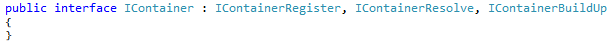
\includegraphics{IContainer.png}
  		\caption{Interfejs IContainer}
  		\label{fig:IContainer}
	\end{center}
\end{figure}
Pierwszy z tych interfejsów to IContainerRegister (Rys. \ref{fig:IContainerRegister}). Zawiera on metody służące do zarejestrowania typów w kontenerze.\\
\begin{figure}[H]
	\begin{center}
  		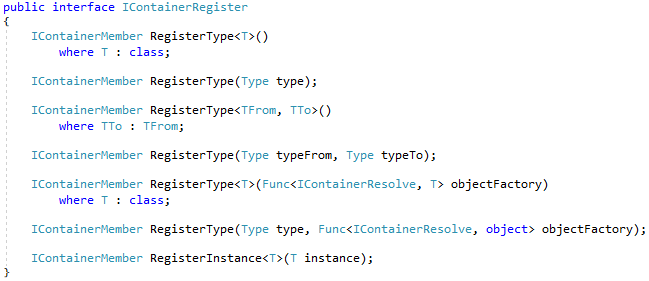
\includegraphics{IContainerRegister.png}
  		\caption{Interfejs IContainerRegister}
  		\label{fig:IContainerRegister}
	\end{center}
\end{figure}
Drugi z nich to IContainerResolve (Rys. \ref{fig:IContainerResolve}). Składa się on z metod odpowiedzialnych za  tworzenie i zwracanie obiektów wcześniej zarejestrowanych typów.\\ \\
\begin{figure}[H]
	\begin{center}
  		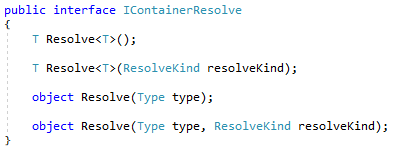
\includegraphics{IContainerResolve.png}
  		\caption{Interfejs IContainerResolve}
  		\label{fig:IContainerResolve}
	\end{center}
\end{figure}
Ostatni z tych interfejsów to IContainerBuildUp (Rys. \ref{fig:IContainerBuildUp}). Jego metody służą do uzupełnienia istniejącej instancji obiektu z wykorzystaniem wstrzykiwania zależności przez metodę i właściwość - są to operacje opcjonalna i nie każde przemysłowe rozwiązanie ją zawiera.\\ \\
\begin{figure}[H]
	\begin{center}
  		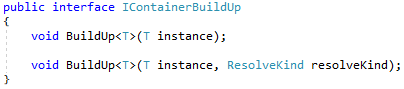
\includegraphics{IContainerBuildUp.png}
  		\caption{Interfejs IContainerBuildUp}
  		\label{fig:IContainerBuildUp}
	\end{center}
\end{figure}
Poniżej znajduje się dokładniejszy opis metod z każdego z powyższych interfejsów.

\subsubsection{Register}
W pierwszej i drugiej metodzie interfejsu IContainerRegister możemy zarejestrować zwykłe klasy. W trzeciej i czwartej interfejsy oraz klasy, które implementują dany interfejs lub klasy i klasy po nich dziedziczące. W piątej i szóstej metodzie rejestrujemy klasę jako fabrykę obiektów - funkcję, która ma nam zwrócić pożądany obiekt. W siódmej (ostatniej) natomiast możemy zarejestrować konkretną instancję danego typu.\\
W moim rozwiązaniu każdy typ może być zarejestrowany tylko raz - ponowna rejestracja tego samego typu nadpisuje istniejącą rejestrację.\\
Każda z tych siedmiu metod rejestracji zwraca interfejs IContainerMember (Rys. \ref{fig:IContainerMember}), który umożliwia nam zarejestrowanie danego typu z określonym menadżerem czasu życia (czyli implementacją interfejsu IObjectLifetimeManager - Rys. \ref{fig:IObjectLifetimeManager}). Zostało to tak zrobione, ponieważ dla różnych przypadków biznesowych możemy potrzebować, aby obiekt danego typu miał konkretny czas życia.\\ \\
\begin{figure}[H]
	\begin{center}
  		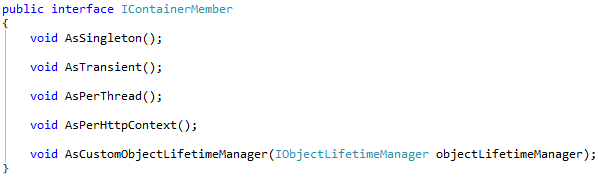
\includegraphics{IContainerMember.png}
  		\caption{Interfejs IContainerMember}
  		\label{fig:IContainerMember}
	\end{center}
\end{figure}
Pierwsze cztery metody interfejsu IContainerMember, to wbudowane implementacje interfejsu IObjectLifetimeManager. Piąta metoda dostarcza możliwość podania przez użytkownika jego własnej implementacji tego interfejsu. W moim rozwiązaniu każdy typ domyślnie ma czas życia Transient.\\
\\
Wyjaśnienie rozdajów czasu życia:
\begin{itemize}
	\item Singleton - za każdym razem zwracany jest ten sam obiekt
	\item Transient - za każdym razem zwracany jest nowy obiekt
	\item PerThread - wewnątrz danego wątku zwracany jest ten sam obiekt, ale dla innego wątku zwracany jest nowy (inny) obiekt
	\item PerHttpContext - wewnątrz danego żądania Http zwracany jest ten sam obiekt, ale dla innego żądania zwracany jest nowy (inny) obiekt
\end{itemize}

W interfejsie IObjectLifetimeManager właściwość ObjectFactory służy do ustawienia funkcji, która zwraca obiekt. Metoda GetInstance służy do pobrania obiektu.\\
W zależności od implementacji tego interfesju, to obiekt zwracany z metody GetInstance może być zawsze taki sam, zawsze różny albo taki sam tylko dla określonych sytuacji (np. taki sam dla tego samego wątku albo tego samego żądania http).\\ \\
\begin{figure}[H]
	\begin{center}
  		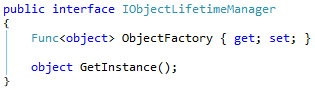
\includegraphics{IObjectLifetimeManager.png}
  		\caption{Interfejs IObjectLifetimeManager}
  		\label{fig:IObjectLifetimeManager}
	\end{center}
\end{figure}

\subsubsection{Resolve}
Metody interfejsu IContainerResolve, są to głównymi operacjami. Register można nazwać sercem kontenera, a Resolve mózgiem. Każda z metod tego interfejsu odpowiada za stworzenie i zwrócenie obiektu odpowiedniego typu.\\
W mojej pracy zaproponowałem dwa rozwiązania - PartialEmitFunction i FullEmitFunction, dlatego te metody jako parametr przyjmuje wartość enuma ResolveKind (dzięki temu w przyszłości może być ona w łatwy sposób rozszerzona o kolejne rozwiązania). W interfejsie znajdują się również metody, które nie przyjmują tego parametru - zostały one dodane na wypadek, gdy ktoś będzie zawsze korzystał tylko z jednego z rozwiązań (może ustawić je jako domyślne np. w konstruktorze).

\subsubsection{BuildUp}
Interfejs IContainerBuildUp to taki dodatek - gdy mamy stworzony obiekt, ale nie jest on w pełni uzupełniony, to możemy go rozbudować (używająć metody z odpowiednią wartością enuma ResolveKind lub tej z wartością domyślną). Z metodami tego interfejsu są powiązane bezpośrednio dwa pojęcia - wstrzykiwanie przez metodę i wstrzykiwanie przez właściwość. Do tego celu w moim rozwiążaniu stworzyłem dwa atrybuty:
\begin{itemize}
	\item DependencyMethod (dla metod)
	\item DependencyProperty (dla właściwości)
\end{itemize}
Podczas operacji BuildUp wywoływane są wszystie metody i uzupełniane są wszystkie właściwości, które mają te atrybuty. Ta operacja jest również wykonywany podczas operacji Resolve.\\

Warto tutaj odnotować, że ze względu na szczegóły implementacyjne tylko jedno z moich rozwiązań wspiera operację BuildUp - jest to rozwiązanie PartialEmitFunction. W rozwiązaniu FullEmitFunction ta funckonalność nie została zaimplementowana. Jest to spowodowane skomplikowaniem tego rozwiązania i małą potrzebą biznesową używania tej operacji. Jednakże w przyszłości istnieje możliwość dodania implementacji tej funkcjonalności.\\

W aplikacji istnieje również atrybut DependencyConstrutor. Można go użyć przy definicji konstruktora danej klasy. Obiekt każdej klasy jest tworzony przy użyciu konstruktora. Klasa może mieć kilka konstruktorów. W moim rozwiązaniu stworzyłem logikę wyboru odpowiedniego konstruktora, przy pomocy którego ma zostać stworzony obiekt. Wygląda ona następująco:
\begin{itemize}
	\item Jeśli jest jeden konstruktor, to go wybierz.
	\item Jeśli jest kilka konstruktorów, to odpowiedni wybierz w poniższej kolejności:
	\begin{enumerate}
		\item Konstruktor z atrybutem DependencyConstrutor
		\item Konstruktor z największą liczbą parametrów
	\end{enumerate}
	\item Jeśli jest kilka konstrutkrów z atrybutem DependencyConstrutor albo nie ma żadnego konstruktora z tym atrybutem i jest kilka z największą liczbą parametrów, to rzuć wyjątek.
\end{itemize}


\subsection{Rozwiązanie}
Stworzenie nowego obiektu zajmuje czas. Gdy graf zależności dla jakiegoś typu jest bardzo rozbudowany, to stworzenie obiektu takiego typu zajmuje dużo czasu. Proces ten można podzielić na trzy etapy:
\begin{itemize}
	\item Uzyskanie informacji jakich typów obiekty są potrzebne do stworzenia danego obiektu.
	\item Stworzenie tych pomocnicznych obiektów.
	\item Stworzenie docelowego obiektu.
\end{itemize}
Gdy mamy rozbudowane grafy zależności, to często zdaża się, że niektóre typy się powtarzają. Zatem pewne informacje możemy uzyskać raz, a następnie je zapamiętać. Aby implementacja wzorca wstrzykiwania zależności działała wydajnie dla złożonych grafów zależności, należy jak najwięcej informacji przechowywać w pamięci podręcznej i należy to robić mądrze.\\
W mojej implementacji stworzyłem dwie strategie, które realizują te założenia. Pierwszy krok jest taki sam dla obu rozwiązań (uzyskanie informacji jakich typów obiekty są potrzebne do stworzenia danego obiektu), natomiast kolejne kroki już się różnią. W pierwszym rozwiązaniu, które nazwałem PartialEmitFunction całym process tworzenia nowego obiektu został rozbity na mniejsze części (docelowy obiekt jest tworzony po kawałku). Każda taka osobna część jest zapisywana w pamięci podręcznej. W drugim rozwiązaniu w pamięci podręcznej jest zapisana tylko jedna operacja. Zawiera ona listę wszystkich kroków, które są niezbędne do stworzenia docelowego obiektu. Więc finalnie docelowy obiekt jest tworzony przy pomocy jednej operacji (kroki drugi i trzeci są połączone). To rozwiązanie nazwałem FullEmitFunction.\\
W obu rozwiązaniach do zapamiętania kroków potrzebnych do stworzenia obiektu danego typu wykorzystałem operacje z przestrzeni nazw Reflection.Emit.

\clearpage
\subsubsection{Krok pierwszy}
Na początku algorytmu znajdujemy odpowiedni konstruktor, przy pomocy którego ma zostać stworzony nowy obiekt. Jeśli robimy to poraz pierwszy dla danego typu, to informację o tym konstruktorze zapisujemy w pamięci podręcznej. Do tego celu została użyta struktura danych Dictionary, gdzie kluczem jest typ obiektu, a wartością obiekt klasy ContainerMember (Rys. \ref{fig:ContainerMember}), w którym przechowujemy wszystkie zapamiętane informacje dla danego typu. Następnym krokiem, jest rekurencyjne wywołanie tej operacji dla wszystkich typów, których obiekty są niezbędne do stworzenia obiektu docelowego typu.\\
W tej operacji jest kilka wyjątków - są nimi typy zarejestrowane jako Instance albo FactoryObject. Dla pierwszego przypadku nie musimy uzyskiwać informacji o tym jak stworzyć obiekt takiego  typu, ponieważ mamy już taki obiekt stworzony i go po prostu wykorzystamy. Dla drugiego przypadku obiekt tworzony jest przy użyciu wcześniej zdefiniowanej przez użytkownika funkcji, której wywołanie spowoduje stworzenie obiektu oczekiwanego typu.\\

Klasa ContainerMember przechowuje:
\begin{itemize}
	\item Informacje o konstruktor, przy pomocy którego należy utworzyć obiekt danego typu.
	\item Informacje o parametrach tego konstruktora.
	\item Informacje o właciwościach danego typu (na potrzeby operacji BuildUp).
	\item Informacje o metodach danego typu (na potrzeby operacji BuildUp).
	\item Czy występuję cykl w konstruktorze.
	\item Przy należy zapamiętać infrmacje dla danego typu (domyślnie tak, dla typóW zarejestrowanych jako Instance albo ObjectFactory - nie).
	\item Zarejestrowany typ (ta sama wartoć, co klucz ze słownika).
	\item Zwracany typ.
	\item Informacje o menadżerze cyklu życia.
\end{itemize}

\begin{figure}[H]
	\begin{center}
  		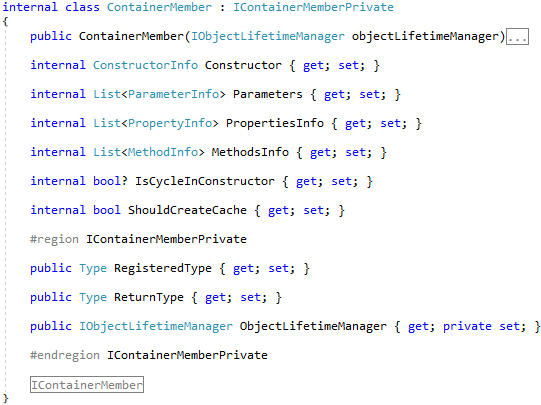
\includegraphics{ContainerMember.png}
  		\caption{Klasa ContainerMember}
  		\label{fig:ContainerMember}
	\end{center}
\end{figure}

\subsubsection{Rozwiązanie 1 - PartialEmitFunction}
Cały algorytm jest zawarty w metodzie Resolve (Rys. \ref{fig:PartialEmitFunction_Resolve}). Sama ta metoda jest dość krótka, ale wywołuje ona kolejne metody (które już są dłuższe).\\
Docelowy obiekt jest tworzony przy pomocy funkcji. Na początku sprawdzamy, czy już wcześniej utworzyliśmy taką funkcję (jeśli tak, będzie on zapisany w klasie ContainerMember we właściwoci ObjectLifetimeManager). Wywołanie funkcji kończy działanie algorytmu. Jeśli funkcja nie została jeszcze wcześniej utworzona, to ją tworzymy.\\
Funkcja ta nie przyjmuje żadnych parametrów, a jej typem wynikowym jest obiekt. Ciało tej funkcji jest bardzo proste - po prostu ma ona wykonać metodę i zwrócić jej rezultat, którym jest nasz docelowy obiekt.\\ \\
\begin{figure}[H]
	\begin{center}
  		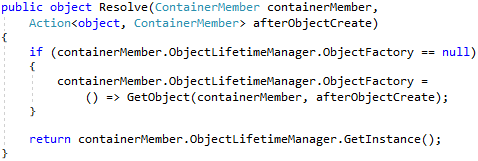
\includegraphics{PartialEmitFunction_Resolve.png}
  		\caption{Metoda Resolve klasy PartialEmitFunction}
  		\label{fig:PartialEmitFunction_Resolve}
	\end{center}
\end{figure}

Metoda GetObject (Rys. \ref{fig:PartialEmitFunction_GetObject}) jest trochę bardziej rozbudowana. Na początku pobieramy informacje o parametrach konstruktora danego typu. Następnie dla każdego z tych parametrów tworzomy obiekt (o docelowym typie) przy pomocy funkcji Resolve (opisanej wyżej). Korzystamy tutaj z rekurencji. Gdy już mamy stworzone obiekty dla każdego z parametrów konstruktora, to listę tych parametrów przekazujemy do metody CreateInstanceFunction, która zwróci nam instancję obiektu oczekiwanego typu. Na koniec wywołujemy callback afterObjectCreate i zwracamy nasz obiekt.\\ \\
\begin{figure}[H]
	\begin{center}
  		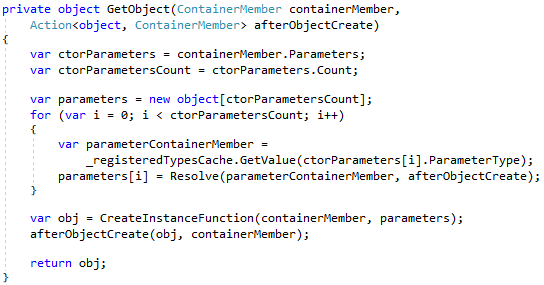
\includegraphics{PartialEmitFunction_GetObject.png}
  		\caption{Metoda GetObject klasy PartialEmitFunction}
  		\label{fig:PartialEmitFunction_GetObject}
	\end{center}
\end{figure}

Na początku metody CreateInstanceFunction (Rys. \ref{fig:PartialEmitFunction_CreateInstanceFunction}) sprawdzamy, czy mamy utworzoną funkcję, która umie zwrócić obiekt docelowego typu. Jeśli tak, to przy pomocy tej funkcji tworzymy obiekt  i go zwracamy. Ta funckja jako argument przyjmuje listę obiektów w kolejności zgodnej z listą parametrów konstruktora. Jeśli nie, to przy pomocy metody CreateObjectFunction tworzymy taką funkcję, a następnie zapisujemy ją w pamięci podręcznej (również w strukturze Dictionary, której kluczem jest type, a wartością jest funkcja).\\ \\
\begin{figure}[H]
	\begin{center}
  		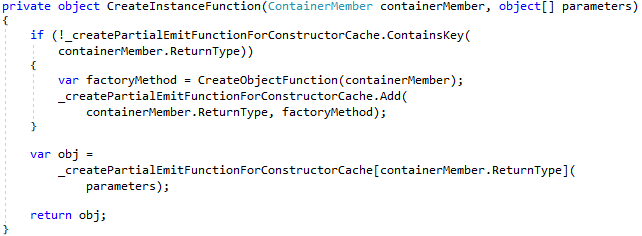
\includegraphics{PartialEmitFunction_CreateInstanceFunction.png}
  		\caption{Metoda CreateInstanceFunction klasy PartialEmitFunction}
  		\label{fig:PartialEmitFunction_CreateInstanceFunction}
	\end{center}
\end{figure}

CreateObjectFunction (Rys. \ref{fig:PartialEmitFunction_CreateObjectFunction}) jest najbardziej zaawansowaną metodą w tym algorytmie. To w niej korzystamy z metod z przestrzeni nazw Reflection.Emit.\\
Na początku pobieramy informacje o konstruktorze. Następnie tworzymy DynamicMethod i z niej pobieramy ILGenerator. W nim będziemy przechowywać listę kroków niezbędnych do utworzenia docelowego obiektu.\\
Dla każdego z parametrów konstruktora wykonujemy następujące operacje:
\begin{enumerate}
	\item Dodaj do listy kroków operację, która umieści na szczycie stosu pierwszy parametr (będzie nim lista obiektów zgodna z parametrami konstruktora).
	\item Dodaj do listy kroków operację, która umieści na szczycie stosu indeks parametru (który to jest parametr z kolei).
	\item Dodaj do listy kroków operację, która zdejmie ze szczytu stosu listę i indeks, a umieści na jego szczycie element znajdujący się pod danym indeksem na liście.
	\item Pobieramy typ parametru.
	\item Dodaj do listy kroków operację, która zrzutuje obiekt ze szczytu stosu na odpowiedni typ.
\end{enumerate}
Po wykonaniu kroków z listy na stosie będziemy mieli wszystkie obiekty, które są wymagane przez konstruktor do utworzenia danego typu. Teraz więc do listy kroków dodajemy operację, która stworzy obiekty przy pomocy danego konstruktora i umieści go na szczycie stosu. Na koniec dodajemy krok, który zwróci nam obiekt ze szczytu stosu.\\
Wszystkie kroki niezbędne do stworzenia nowego elementu są zapisane w zmiennej typu DynamicMethod. Jako ostatnią operację w metodzie CreateObjectFunction, ze zmiennej typu DynamicMethod, tworzymy i zwracamy delegata, który jako parametr będzie przyjmował tablicę obiektów (nasza lista obiektów zgodna z parametrami konstruktora), a zwracał obiekt (nasz docelowy obiekt).\\ \\
\begin{figure}[H]
	\begin{center}
  		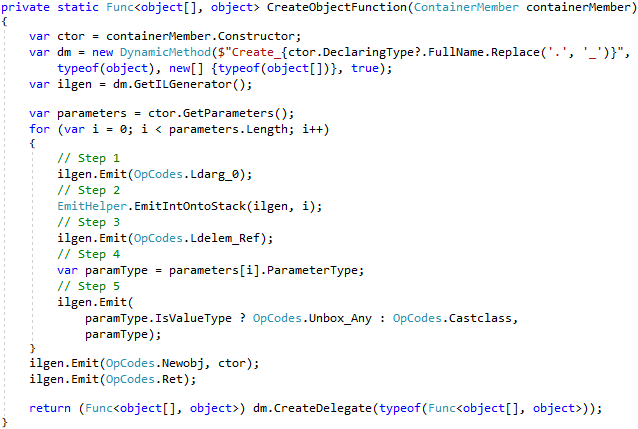
\includegraphics{PartialEmitFunction_CreateObjectFunction.png}
  		\caption{Metoda CreateObjectFunction klasy PartialEmitFunction}
  		\label{fig:PartialEmitFunction_CreateObjectFunction}
	\end{center}
\end{figure}

\subsubsection{Rozwiązanie 2 - FullEmitFunction}
Tutaj podobnie jak dla PartialEmitFunction cały algorytm zawarty jest w metodzie Resolve (Rys. \ref{fig:FullEmitFunction_Resolve}). Wygląda ona identycznie jak w rozwiązaniu 1 - docelowy obiekt jest tworzony przy pomocy funkcji, która woła w sobię metodę GetObject. Jeśli funkcji nie ma w zapisanej w pamięci, to ją tworzymy i zapisuje. Na końcu ją wywołujemy.\\ \\
\begin{figure}[H]
	\begin{center}
  		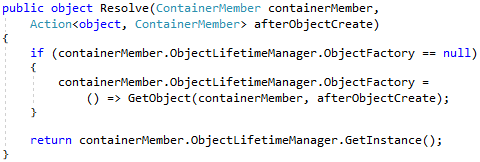
\includegraphics{FullEmitFunction_Resolve.png}
  		\caption{Metoda Resolve klasy FullEmitFunction}
  		\label{fig:FullEmitFunction_Resolve}
	\end{center}
\end{figure}

Metoda GetObject (Rys. \ref{fig:FullEmitFunction_GetObject}) wygląda trochę inaczej. Nie pobieramy tutaj żadnych dodatkowych informacji, tylko od razu wywołujemy metodę CreateInstanceFunction, która zwróci nam instancję obiektu oczekiwanego typu. Na koniec również wywołujemy callback afterObjectCreate i zwracamy nasz obiekt.\\ \\
\begin{figure}[H]
	\begin{center}
  		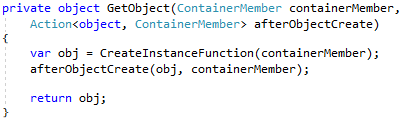
\includegraphics{FullEmitFunction_GetObject.png}
  		\caption{Metoda GetObject klasy FullEmitFunction}
  		\label{fig:FullEmitFunction_GetObject}
	\end{center}
\end{figure}

CreateInstanceFunction (Rys. \ref{fig:FullEmitFunction_CreateInstanceFunction}) ma jeden dodatkowy krok względem rozwiązania 1. Na początku również sprawdzamy, czy mamy utworzoną funkcję, która umie zwrócić obiekt docelowego typu. Jeśli nie, to przy pomocy metody CreateObjectFunction tworzymy taką funkcję, a następnie zapisujemy ją w pamięci podręcznej (również w strukturze Dictionary, której kluczem jest type, a wartością jest typ pomocniczy FullEmitFunctionResult, który ma tylko jedną właściwość - Result typu funkcja). Następnym krokiem jest zwalidowanie zapisanych danych dla typów przy pomocy metody ValidateTypesCache. Na końcu funkcji tworzymy obiekt  i go zwracamy. Tutaj funckja jako argument przyjmuje dwa słowniki. Pierwszy zawiera informacje o typie (kluczem jest typ, a wartością obiekt ContainerMember), a drugi informacje o indeksie typu (kluczem jest liczba oznaczając hasz danego typu, a wartością typ).\\
Najpierw opiszę metodę ValidateTypesCache, ponieważ nie wywołuje ona w sobie żadnej innej metody.\\ \\
\begin{figure}[H]
	\begin{center}
  		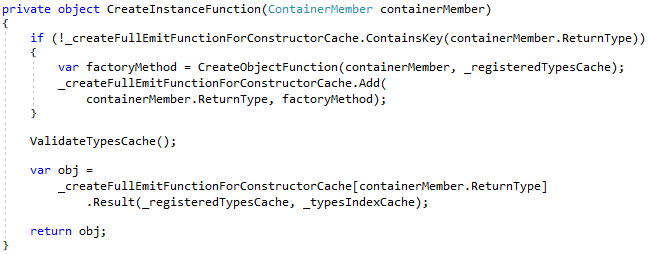
\includegraphics{FullEmitFunction_CreateInstanceFunction.png}
  		\caption{Metoda CreateInstanceFunction klasy FullEmitFunction}
  		\label{fig:FullEmitFunction_CreateInstanceFunction}
	\end{center}
\end{figure}

W pierwszym kroku metody ValidateTypesCache sprawdzamy (Rys. \ref{fig:FullEmitFunction_ValidateTypesCache}), czy od ostatniego zapisywania danych o typach w pamięci podręcznej jakiś typ został zarejestorwany w kontenerze (lub czy jest to pierwsze zapisanie tych danych). Jeśli tak, to tworzymy z zarejestrowanych typów tworzymy słownik, w którym kluczem jest hasz typu, a wartością typ. Potem aktualizujemy liczbę aktualnie zarejestrowanych typów.\\ \\
\begin{figure}[H]
	\begin{center}
  		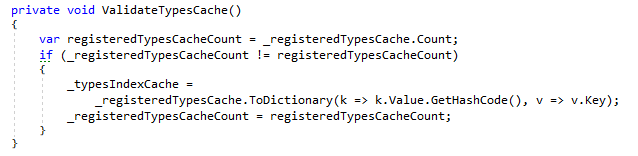
\includegraphics{FullEmitFunction_ValidateTypesCache.png}
  		\caption{Metoda ValidateTypesCache klasy FullEmitFunction}
  		\label{fig:FullEmitFunction_ValidateTypesCache}
	\end{center}
\end{figure}

Metoda CreateObjectFunction (Rys. \ref{fig:FullEmitFunction_CreateObjectFunction}) jest dużo bardziej rozbudowana niż w rozwiązaniu 1. W niej również korzystamy z metod z przestrzeni nazw Reflection.Emit.\\
Na początku tworzymy DynamicMethod i z niej pobieramy ILGenerator, w którym będziemy przechowywać listę kroków niezbędnych do utworzenia docelowego obiektu.\\
Dla każdego z parametrów konstruktora wywołujemy metodę CreateObjectFunctionPrivate, która uzupełni listę kroków o tworzenie pośrednich obiektów. To w tym miejscu jest główna różnica między oboma rozwiązaniami - w pierwszym rozwiązaniu w liście kroków nie przejmowaliśmy się utworzeniem pośrednich obiektów, ponieważ przychodziły one jako parametr. W tym rozwiązaniu lista kroków będzie również zawierać kroki do utworzenia wszystkich obiektów pośrednich (obiektów wymaganych przez konstruktory).\\
Dalsze operacje są takie same jak w rozwiązaniu 1 - do listy kroków dodajemy operację, która stworzy obiekty przy pomocy danego konstruktora i umieści go na szczycie stosu, a następnie dodajemy operację, który zwróci nam obiekt ze szczytu stosu.\\
Na końcu ze zmiennej typu DynamicMethod tworzymy delegata i go zwracamy. Delegat będzie przyjmował dwa parametry - oba typu Dictionaty. Jeden z informacjami o type, a drugi z informacjiami o indeksie typu.\\ \\
\begin{figure}[H]
	\begin{center}
  		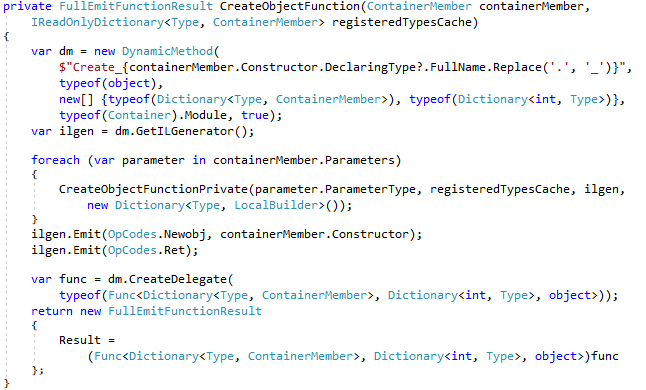
\includegraphics{FullEmitFunction_CreateObjectFunction.png}
  		\caption{Metoda CreateObjectFunction klasy FullEmitFunction}
  		\label{fig:FullEmitFunction_CreateObjectFunction}
	\end{center}
\end{figure}

W metodzie CreateObjectFunctionPrivate (Rys. \ref{fig:FullEmitFunction_CreateObjectFunctionPrivate}) mamy trzy przypadki. W pierwszych dwóch przypadkach pomijamy obiekty, które zostały zarejestrowane jako Instance albo FactoryObject (określa to parametr ShouldCreateCache z obiektu typu ContainerMember).\\
\begin{figure}[H]
	\begin{center}
  		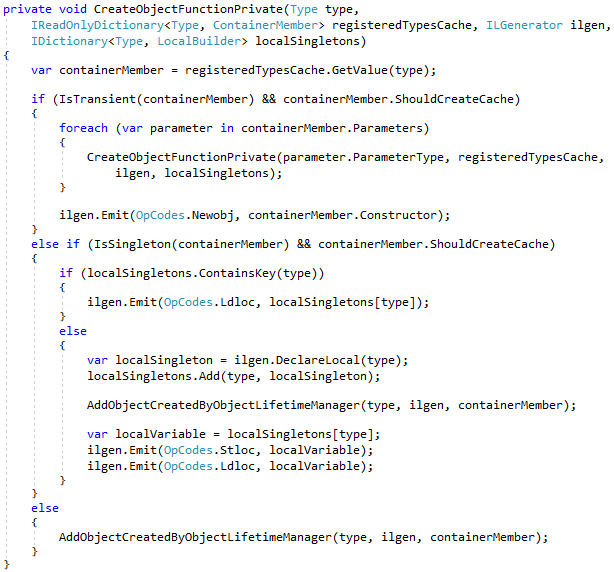
\includegraphics{FullEmitFunction_CreateObjectFunctionPrivate.png}
  		\caption{Metoda CreateObjectFunctionPrivate klasy FullEmitFunction}
  		\label{fig:FullEmitFunction_CreateObjectFunctionPrivate}
	\end{center}
\end{figure}

Pierwszy przypadek, to gdy typ został zarejestrowany jako Transient -  Rys. \ref{fig:FullEmitFunction_IsTransient}. Wtedy dla każdego z parametrów konstruktora wywołujemy rekurencyjnie tę metodę (CreateObjectFunctionPrivate), a na koniec do listy kroków dodajemy operację, która stworzy obiekty przy pomocy danego konstruktora i umieści go na szczycie stosu.\\ \\
\begin{figure}[H]
	\begin{center}
  		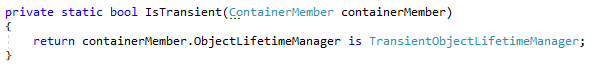
\includegraphics{FullEmitFunction_IsTransient.png}
  		\caption{Metoda IsTransient klasy FullEmitFunction}
  		\label{fig:FullEmitFunction_IsTransient}
	\end{center}
\end{figure}

W drugim przypadeku typ musi być singletonem (został on zarejestrowany jako Singleton, PerThread lub PerHttpContext) -  Rys. \ref{fig:FullEmitFunction_IsSingleton}. Na początku sprawdzamy czy już wcześniej natrafiliśmy na ten typ. Jeśli tak, to z pamięci podręcznej pobieramy zmienną lokalną dla danego typu, a następnie do listy kroków dodajemy operację, która doda na szczyt stosu obiekt z tej zmiennej. Jeśli nie, to najpierw tworzymy nową zmienną lokalną dla danego typu i zapisuje ją w pamięci podręcznej (wykorzystujemy do tego słownik, gdzie kluczem jest typ, a wartością obiekt typu LocalBuilder). Następnie wywołujemy metodę AddObjectCreatedByObjectLifetimeManager. Na końcu dodajemy dwie operacje. Pierwsza z nich zdejmie obiekt ze szczytu stosu i zapisze go w zmiennej lokalnej, a druga umieści na szczycie stosu obiekt z tej zmiennej lokalnej. Jest to po to, ponieważ na szczycie stosu chcemy mieć dany obiekt, ale również chcemy zapamiętać sobie dany obiekt, aby nie trzeba było go tworzyć, jeśli będzie potrzebny poraz drugi (obiekt jest singletonem, więc za każdym razem będziemy chcieli mieć ten sam obiekt - w kontekście tworzenia danego typu, czyli jednej operacji Resolve).\\ \\
\begin{figure}[H]
	\begin{center}
  		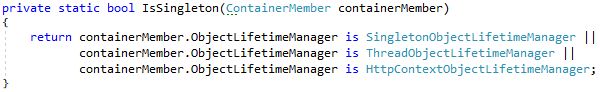
\includegraphics{FullEmitFunction_IsSingleton.png}
  		\caption{Metoda IsSingleton klasy FullEmitFunction}
  		\label{fig:FullEmitFunction_IsSingleton}
	\end{center}
\end{figure}

Metoda AddObjectCreatedByObjectLifetimeManager (Rys. \ref{fig:FullEmitFunction_AddObjectCreatedByObjectLifetimeManager}), za wyjątkiem pierwszej operacji jaką jest stworzenie zmiennej lokalnej typu Type, zawiera jedynie operacje, które dodają kolejne pozycje do listy kroków:
\begin{enumerate}
	\item Dodaj do listy kroków operację, która umieści na szczycie stosu drugi parametr (będzie nim słownik z indeksami typów).
	\item Dodaj do listy kroków operację, która umieści na szczycie stosu hasz danego typu.
	\item Dodaj do listy kroków operację, która pobierze ze szczytu stosu słownik i indeks, a umieści na jego szczycie element znajdujący się pod danym kluczem w słowniku.
	\item Dodaj do listy kroków operację, która zdejmie obiekt ze szczytu stosu i zapisze go w zmiennej lokalnej.
	\item Dodaj do listy kroków operację, która umieści na szczycie stosu pierwszy parametr (będzie nim słownik z informacjami o typach).
	\item Dodaj do listy kroków operację, która umieści na szczycie stosu obiekt ze zmiennej lokalnej.
	\item Dodaj do listy kroków operację, która zdejmie ze szczytu stosu słownik i typ, a umieści na jego szczycie element znajdujący się pod danym kluczem w słowniku.
	\item Dodaj do listy kroków operację, która zdejmie obiekt ze szczytu stosu (będzie to obiekt typu ContainerMember), wywoła na nim metodę, która zwróci menadżer czasu życia obiektu i na szczycie stosu umieści rezultat tej metody.
	\item Dodaj do listy kroków operację, która zdejmie obiekt ze szczytu stosu (będzie to obiekt typu IObjectLifeTimeManager), wywoła na nim metodę, która zwróci instancję obiektu i na szczycie stosu umieści rezultat tej metody.
	\item Dodaj do listy kroków operację, która zrzutuje obiekt ze szczytu stosu na odpowiedni typ.
\end{enumerate}
Po wykonaniu tych 10 operacji na szczycie stosu znajdzie się obiekt danego typu utworzony przy pomocy menadżera czasu życia.\\ \\
\begin{figure}[h]
	\begin{center}
  		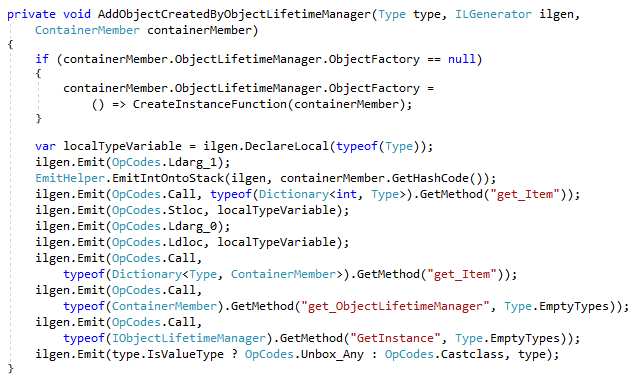
\includegraphics{FullEmitFunction_AddObjectCreatedByObjectLifetimeManager.png}
  		\caption{Metoda AddObjectCreatedByObjectLifetimeManager klasy FullEmitFunction}
  		\label{fig:FullEmitFunction_AddObjectCreatedByObjectLifetimeManager}
	\end{center}
\end{figure}

Trzeci przypadek zachodzi gdy typ został zarejestrowany jako Instance, FactoryObject lub przy pomocy własnego menadżera czasu życia (implementacji interfejsu IObjectLifetimeManager). W tej sytuacji wywołujemy po prostu metodę AddObjectCreatedByObjectLifetimeManager.



\clearpage
\section{Testy wydajnościowe}
Do przeprowadzania testów wydajnościowych stworzyłem osobną aplikację w której utworzyłem 4 przypadki testowe:
\begin{itemize}
	\item Przypadek testowy A,
	\item Przypadek testowy B,
	\item Przypadek testowy C,
	\item Przypadek testowy D.
\end{itemize}
Dla każdego z przypadków sprawdzany jest czas wykoniania operacji "Register" i "Resolve" dla różnych rodzajów rejestracji. Testy zostały wykonane dla następujących wariantów rejestracji:
\begin{itemize}
	\item Register as Singleton,
	\item Register as Transient,
	\item Register as TransientSingleton,
	\item Register as PerThread (dla niektórych przemysłowych rozwiązań - PerScope),
	\item Register as FactoryMethod.
\end{itemize}
Każdy z testów dla każdego rozwiązania był uruchamiany w osobnym procesie. Najpierw zostaną zaprezentowane czasy dla operacji "Register" dla wszystkich rozdajów rejestracji, a następnie dla każdego z rodzaju czasy dla operacji "Resolve". Wynika to z tego, że czasy dla rejestracji są prawie zawsze zbliżone do 0. Ze względu na nieduży narzut czasu, te testy zostały uruchamiane tylko 1 raz. Przy operacji "Resolve" każdy test był uruchamiany 100 razy, a w wynikach zostały przedstawione następujące czasy w milisekundach: minimalny, maksymalny i średni. Dla pierwszych trzech przypadków testy były wykonywane dla: 1, 10, 100 i 1000 powtórzeń, a dla ostatniego przypadku dla: 1 i 10 powtórzeń. Spowodowane jest to ilością obiektów, które są tworzone jednorazowo dla poszczególnych przypadków testowych.

\subsubsection{Register as Singleton}
Każdy typ jest zarejestrowany jako "Singleton", czyli obiekt jest tworzony raz, a następnie cały czas zwracany.

\subsubsection{Register as Transient}
Każdy typ jest zarejestrowany jako "Transient", czyli za każdym razem jest tworzony nowy obiekt.

\subsubsection{Register as TransientSingleton}
Każdy typ jest zarejestrowany jako "Transient" za wyjątkiem typów, które maja konstruktor bezparametrowy - są one zarejestrowane jako "Singleton".

\subsubsection{Register as PerThread}
Każdy typ jest zarejestrowany jako "PerThread", czyli obiekt jest tworzony raz dla każdego wątku, a następnie w obrębie tego wątku cały czas zwracany.

\subsubsection{Register as FactoryMethod}
Każdy typ jest zarejestrowany jako "FactoryMethod", czyli jako funkcja, która zwraca nam obiekt danego typu. Ciało tej funkcji wygląda tak, że oczekiwany typ jest tworzony z użyciem konstruktora (za pomocą "new"), a wszystkie parametry wymagane przez ten konstruktor są tworzone przy pomocy operacji Resolve.


\subsection{Przypadek testowy A}
\subsubsection{Opis}
W tym teście mamy zdefiniowanych 11 typów. Każdy z nich przymuje w konstruktorze o jeden parametr mniej niż typ poprzedni (czyli przyjmują one kolejno od 10 do 0 parametrów w konstruktorze). Typem głównym, a zarazem typem o największej liczbie parametrów, jest typ "TestA". Przyjmuje on w konstruktorze 10 parametrów następujących typów: "TestA0", "TestA1", "TestA2", "TestA3", "TestA4", "TestA5", "TestA6", "TestA7", "TestA8", "TestA9". Każdy z tych 10 typów w konstruktorze przyjmuje tyle parametrów, jaki ma numerek w nazwie (czyli obiekt typu "TestA0" ma konstruktore bezparametrowy, obiekt typy "TestA1" ma konstuktor z jednym parametrem; i tak dalej aż do typu "TestA9", który ma konstruktor z dziewięcioma parametrami). Wszystkie typy jako parametry w konstruktorze przyjmuje obiekty typów z niższymi numerkami (czyli obiekt typu "TestA1" w konstruktorze przyjmuje obiekt typu "TestA0", obiekt typu "TestA2" przymuje w konstruktorze obiekty typóW "TestA0" i "TestA1";  i tak dalej aż do typu "TestA9", który w konstruktorze przyjmuje obiekty z typami od "TestA0" do "TestA8"). Graf zależności poszczególnych typów został przedstawiony na Rys. \ref{fig:testA}.\\
\begin{figure}[H]
	\begin{center}
  		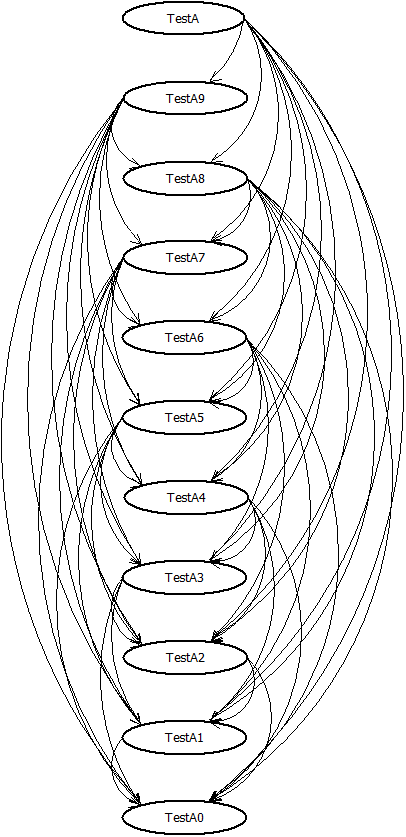
\includegraphics[height=11.5cm]{TestA.png}
  		\caption{Graf zależności dla testu A.}
  		\label{fig:testA}
	\end{center}
\end{figure}

Łatwo z niego wywnioskować, że tworząc obiekty poszczególnych typów ilość tworzonych obiektów rośnie dwukrotnie:
\begin{itemize}
	\item TestA0 - 1 obiekt,
	\item TestA1 - 2 obiekty (obiekt typu TestA1 i obiekt typu TestA0),
	\item TestA2 - 4 obiekty (obiekt typu TestA2, obiekt typu TestA1 - 2 obiekty, obiekt typu TestA0 - 1 obiekt),
	\item TestA3 - 8 obiektów (obiekt typu TestA3, obiekt typu TestA2 - 4 obiekty, obiekt typu TestA1 - 2 obiekty, obiekt typu TestA0 - 1 obiekt),
	\item TestA4 - 16 obiektów,
	\item TestA5 - 32 obiektów,
	\item TestA6 - 64 obiektów,
	\item TestA7 - 128 obiektów,
	\item TestA8 - 256 obiektów,
	\item TestA9 - 512 obiektów,
	\item TestA - 1 024 obiektów.
\end{itemize}
Zatem tworząc nasz główny obiekt typu TestA, tworzymy: 1 obiekt typu TestA, 1 obiekt typu TestA9, 2 obiekty typu TestA8, 4 obiekty typu TestA7, 8 obiektów typu TestA6, 16 obiektów typu TestA5, 32 obiektów typu TestA4, 64 obiektów typu TestA3, 128 obiektów typu TestA2, 256 obiektów typu TestA1 i 512 obiektów typu TestA0 - co w sumie daje 1024 obiekty.

\subsubsection{Wyniki dla Register}
\begin{table}[H]
\captionsetup{belowskip=0pt,aboveskip=0pt}
\begin{center}
\begin{small}
	\begin{tabular}{ | l | r | r | r | r | }
    		\hline
Test & Singleton & Transient & TransientSingleton & PerThread \\ \hline
Autofac & 0 & 0 & 0 & 0 \\ \hline
DryIoc & 0 & 0 & 0 & 0 \\ \hline
Grace & 0 & 0 & 0 & 0 \\ \hline
LightInject & 0 & 0 & 0 & 0 \\ \hline
Ninject & 0 & 0 & 0 & 0 \\ \hline
NiquIoCPartial & 0 & 0 & 0 & 0 \\ \hline
NiquIoCFull & 0 & 0 & 0 & 0 \\ \hline
SimpleInjector & 0 & 0 & 0 & 0 \\ \hline
StructureMap & 0 & 0 & 0 & 0 \\ \hline
Unity & 0 & 0 & 0 & 0 \\ \hline
Windsor & 0 & 0 & 0 & 0 \\ \hline
  	\end{tabular}
\end{small}
\end{center}
\caption{Wyniki testów dla operacji Register dla Przypadku testowego A}
\label{TestCaseA_Register}
\end{table}
Dla każdego z rozwiązań, dla wszystkich testów w tym przypadku testowym, czasy rejestracji są równe 0, czyli poniżej 1 ms.

\subsubsection{Wyniki dla Singleton}
\begin{table}[H]
\captionsetup{belowskip=0pt,aboveskip=0pt}
\begin{center}
\begin{small}
	\begin{tabular}{ | l | r r r | r r r | r r r | r r r | }
    		\hline
Ilość & & 1 & & & 10 & & & 100 & & & 1000 & \\ \hline
 & min & max & avg & min & max & avg & min & max & avg & min & max & avg \\ \hline
Autofac & 0 & 0 & 0 & 0 & 0 & 0 & 0 & 0 & 0 & 0 & 0 & 0 \\ \hline
DryIoc & 2 & 2 & 2 & 2 & 2 & 2 & 2 & 2 & 2 & 2 & 2 & 2 \\ \hline
Grace & 2 & 2 & 2 & 2 & 2 & 2 & 2 & 2 & 2 & 2 & 3 & 2 \\ \hline
LightInject & 2 & 2 & 2 & 2 & 2 & 2 & 2 & 2 & 2 & 2 & 2 & 2 \\ \hline
Ninject & 3 & 3 & 3 & 3 & 3 & 3 & 3 & 3 & 3 & 6 & 7 & 6 \\ \hline
NiquIoCPartial & 1 & 1 & 1 & 1 & 1 & 1 & 1 & 1 & 1 & 1 & 1 & 1 \\ \hline
NiquIoCFull & 2 & 2 & 2 & 2 & 2 & 2 & 2 & 3 & 2 & 2 & 2 & 2 \\ \hline
SimpleInjector & 2 & 2 & 2 & 2 & 2 & 2 & 2 & 2 & 2 & 2 & 2 & 2 \\ \hline
StructureMap & 9 & 10 & 9 & 9 & 10 & 9 & 9 & 10 & 9 & 10 & 11 & 10 \\ \hline
Unity & 7 & 8 & 7 & 7 & 8 & 7 & 7 & 8 & 7 & 8 & 8 & 8 \\ \hline
Windsor & 0 & 0 & 0 & 0 & 0 & 0 & 0 & 0 & 0 & 0 & 0 & 0 \\ \hline
  	\end{tabular}
\end{small}
\end{center}
\caption{Wyniki testów dla operacji Singleton dla Przypadku testowego A}
\label{TestCaseA_Singleton}
\end{table}
Dla tego testu najlepiej poradziły sobie dwa z najpopularniejszych rozwiązania - Aurofac i Windsor. Rozwiązanie NiquIoCPartial uplasowało się na 3 miejscu. Najsłabiej poradził sobie pozostałe najpopularniejsze rozwiązania: Ninject, Unity oraz StructureMap. Reszta rozwiązań miała zbliżone czasy - dwukrotnie większe niż NiquIoCPartial i trzykrotnie mniejsze niż Ninject.

\subsubsection{Wyniki dla Transient}
\begin{table}[H]
\captionsetup{belowskip=0pt,aboveskip=0pt}
\begin{center}
\begin{small}
	\begin{tabular}{ | l | r r r | r r r | r r r | r r r | }
    		\hline
Ilość & & 1 & & & 10 & & & 100 & & & 1000 & \\ \hline
 & min & max & avg & min & max & avg & min & max & avg & min & max & avg \\ \hline
Autofac & 0 & 0 & 0 & 6 & 7 & 6 & 58 & 63 & 59 & 584 & 609 & 587 \\ \hline
DryIoc & 14 & 14 & 14 & 14 & 15 & 15 & 16 & 16 & 16 & 29 & 30 & 29 \\ \hline
Grace & 15 & 16 & 15 & 15 & 16 & 16 & 18 & 19 & 18 & 37 & 38 & 37 \\ \hline
LightInject & 10 & 10 & 10 & 10 & 10 & 10 & 11 & 12 & 11 & 19 & 20 & 19 \\ \hline
Ninject & 10 & 12 & 11 & 88 & 95 & 90 & 864 & 1035 & 882 & 8745 & 9610 & 8934 \\ \hline
NiquIoCPartial & 1 & 1 & 1 & 3 & 3 & 3 & 19 & 22 & 19 & 171 & 198 & 173 \\ \hline
NiquIoCFull & 8 & 9 & 8 & 8 & 9 & 8 & 9 & 10 & 9 & 18 & 19 & 18 \\ \hline
SimpleInjector & 13 & 14 & 13 & 13 & 14 & 14 & 15 & 15 & 15 & 28 & 30 & 29 \\ \hline
StructureMap & 10 & 10 & 10 & 13 & 14 & 14 & 53 & 55 & 54 & 414 & 457 & 417 \\ \hline
Unity & 8 & 9 & 8 & 16 & 17 & 16 & 88 & 91 & 88 & 803 & 961 & 813 \\ \hline
Windsor & 1 & 2 & 1 & 16 & 21 & 16 & 152 & 192 & 155 & 1511 & 1799 & 1529 \\ \hline
  	\end{tabular}
\end{small}
\end{center}
\caption{Wyniki testów dla operacji Transient dla Przypadku testowego A}
\label{TestCaseA_Transient}
\end{table}
W tym teście jest już spora rozbieżność czasów. Gdy mamy tylko 1 operację najlepiej radzi sobie Autofac, a zaraz za nim NiquIoCPartial i Windsor. Najsłabiej natomiast SimplyInjector, DryIoc i Grace. Pozostałe rozwiązania wypadły przeciętnie i bliżej im było do czasów najgorszych, niż najlepszych.\\
Dla 10 operacji sytuacja zaczyna się lekko zmieniać. Tym razem znacząco najlepiej radzi sobie NiquIoCPartial - ponad dwa razy lepiej niż drugi Autofac. Kolejne miejsca należą do NiquIoCFull i LightInject. Pozostałe rozwiązania miały podobne, trochę słabsze czasy. Wyjątkiem jest jedynie Ninject, który poradził sobie najgorzej i jego czas jest ponad 5 razy większy niż dla rozwiązania z przedostatnim czasem (Windsor).\\
Przy 100 operacji na prowadzenie wysuneły się mniej popularne rozwiązania. Na pierwszym miejscu jest NiquIoCFull, a kolejne miejsca to LightInject i SimpleInjector. DryIoc, Grace oraz NiquIoCPartial wypadły akceptowalnie - poradziły sobie trochę gorzej niż trzeci SimpleInjector. Do grona najsłabszych (Unity, Windsor, Ninject) w tym przypadku dołączył również Autofac, który z drugiego miejsca spadł na ósme. StructureMap miał czasy tylko trochę lepszy niż Autofac.\\
Natomiast dla 1000 operacji od czołówki oddalił się NiquIoCPartial. Na pierwszym miejscu wciąż pozostaje NiquIoCFull, a zaraz za nim LightInject i SimpleInjector. DryIoc i Grace wciąż tochę słabiej, ale nadal zadowalająco. Pozostałe rozwiązania mają czasy od kilku do kilkunastu razy gorsze niż reszta. Bez cienia wątpliwości najgorzej wypadł Ninjec.\\
Warto tutaj zaznaczyć, że wraz ze wzrostem operacji najmniejszy wzorst czasów miały rozwiązania: LightInject, NiquIoCFull, SimpleInjector, DryIoc oraz Grace.

\subsubsection{Wyniki dla TransientSingleton}
\begin{table}[H]
\captionsetup{belowskip=0pt,aboveskip=0pt}
\begin{center}
\begin{small}
	\begin{tabular}{ | l | r r r | r r r | r r r | r r r | }
    		\hline
Ilość & & 1 & & & 10 & & & 100 & & & 1000 & \\ \hline
 & min & max & avg & min & max & avg & min & max & avg & min & max & avg \\ \hline
Autofac & 0 & 0 & 0 & 6 & 7 & 6 & 53 & 62 & 54 & 531 & 561 & 535 \\ \hline
DryIoc & 18 & 19 & 18 & 19 & 19 & 19 & 20 & 21 & 20 & 31 & 32 & 32 \\ \hline
Grace & 9 & 10 & 10 & 10 & 10 & 10 & 10 & 11 & 11 & 18 & 19 & 18 \\ \hline
LightInject & 14 & 15 & 14 & 14 & 14 & 14 & 14 & 15 & 15 & 20 & 21 & 20 \\ \hline
Ninject & 9 & 10 & 10 & 65 & 82 & 67 & 626 & 743 & 641 & 6297 & 7218 & 6463 \\ \hline
NiquIoCPartial & 1 & 1 & 1 & 2 & 3 & 2 & 14 & 15 & 14 & 120 & 123 & 121 \\ \hline
NiquIoCFull & 5 & 6 & 5 & 5 & 6 & 5 & 6 & 6 & 6 & 10 & 12 & 11 \\ \hline
SimpleInjector & 9 & 9 & 9 & 9 & 10 & 9 & 10 & 11 & 10 & 17 & 19 & 17 \\ \hline
StructureMap & 9 & 10 & 10 & 12 & 12 & 12 & 35 & 40 & 36 & 252 & 306 & 256 \\ \hline
Unity & 8 & 9 & 8 & 14 & 15 & 14 & 73 & 82 & 74 & 659 & 753 & 663 \\ \hline
Windsor & 1 & 2 & 1 & 12 & 14 & 12 & 117 & 140 & 119 & 1161 & 1302 & 1177 \\ \hline
  	\end{tabular}
\end{small}
\end{center}
\caption{Wyniki testów dla operacji TransientSingleton dla Przypadku testowego A}
\label{TestCaseA_TransientSingleton}
\end{table}
Przy tym teście dla 1 operacji również najlepiej poradziły sobie Autofac, NiquIoCPartial i Windsor. Trochę gorzej NiquIoCFull. Czasy dla Unity, SimpleInjector, Grace, StructureMap i Ninject są zbliżone, jednak duże. Najgorzej wypadły natomiast LightInject i DryIoc.\\
Gdy mamy 10 operacji na drugie miejsce wskoczył NiquIoCFull. Na pierwsze przesunął się NiquIoCPartial, a Autofac spadł na trzecie. Kolejne miejsce zajmują SimpleInjector i Grace. Trochę gorzej poradził sobie StrutureMap. Zaraz za nim jest Windsor, który z podium spadł na 7 miejsce. Kolejne miejsca to LightInject i Unity. DryIoc nadal słabo, jednakże wzrostu czasu był nieduży. Ostatnie miejsce zajął Ninject.\\
Dla 100 operacji na pierwszym miejscu znalazł się NiquIoCFull. Na podium znaleźli się jeszcze SimpleInjector i Grace. NiquIoCPartial spadł poza podium, a tuż za nim jest LightInject. DryIoc nadal z niedużym wzrostem czasu i tym razem jego wynik jest już akceptowalny. Pozostałe rozwiążań bardzo słabo. Kolejne miejsca to StructureMap oraz Autofac, a ranking zamykają Unity, Windsor i Ninject.\\
Test dla 1000 operacji nie spowodował żadnych zmiań w rankingu. Jedynie różnica czasów pomiędzy pierwszą 5, a pozostały miejscami znacząco się zwiększyła. Dla pierwszej piątki czasy zwrosły około dwukrotkie, a dla pozostały miejsc ponad siedmiokrotnie.

\subsubsection{Wyniki dla PerThread}
\begin{table}[H]
\captionsetup{belowskip=0pt,aboveskip=0pt}
\begin{center}
\begin{small}
	\begin{tabular}{ | l | r r r | r r r | r r r | r r r | }
    		\hline
Ilość & & 1 & & & 10 & & & 100 & & & 1000 & \\ \hline
 & min & max & avg & min & max & avg & min & max & avg & min & max & avg \\ \hline
Autofac & 0 & 0 & 0 & 0 & 0 & 0 & 0 & 0 & 0 & 0 & 0 & 0 \\ \hline
DryIoc & 71 & 73 & 71 & 71 & 72 & 71 & 71 & 73 & 72 & 72 & 74 & 72 \\ \hline
Grace & 4 & 4 & 4 & 4 & 4 & 4 & 4 & 4 & 4 & 4 & 4 & 4 \\ \hline
LightInject & 50 & 53 & 50 & 50 & 51 & 50 & 50 & 54 & 51 & 50 & 52 & 51 \\ \hline
Ninject & 3 & 3 & 3 & 3 & 3 & 3 & 3 & 3 & 3 & 6 & 7 & 6 \\ \hline
NiquIoCPartial & 1 & 1 & 1 & 1 & 1 & 1 & 1 & 1 & 1 & 1 & 1 & 1 \\ \hline
NiquIoCFull & 2 & 2 & 2 & 2 & 2 & 2 & 2 & 3 & 2 & 2 & 2 & 2 \\ \hline
SimpleInjector & 7 & 8 & 8 & 8 & 8 & 8 & 8 & 8 & 8 & 8 & 8 & 8 \\ \hline
StructureMap & 9 & 10 & 9 & 9 & 10 & 9 & 9 & 10 & 9 & 10 & 10 & 10 \\ \hline
Unity & 7 & 8 & 7 & 7 & 8 & 7 & 7 & 8 & 7 & 8 & 9 & 8 \\ \hline
Windsor & 0 & 0 & 0 & 0 & 0 & 0 & 0 & 0 & 0 & 0 & 0 & 0 \\ \hline
  	\end{tabular}
\end{small}
\end{center}
\caption{Wyniki testów dla operacji PerThread dla Przypadku testowego A}
\label{TestCaseA_PerThread}
\end{table}
Czasy dla tego przypadku powinny być zbliżone do czasów dla przypadku Singleton, ponieważ wszystko było uruchamiane w jednym wątku. Niestety część rozwiązań sobie z tym nie poradziła.\\
Wyniki zbliżone posiadają: Autofac, Grace, Ninject, NiquIoCPartial, NiquIoCFull, StructureMap, Unity i Windsor. Natomiast dla SimpleInjector, LightInject i DryIoC czasy są od kilku do nawet kilkudziesięciu razy większe.\\
Jeśli chodzi o najlepsze rozwiązania, to wyglądają one tak samo jak dla Singleton. Pierwsze trzy miejsca to Aurofac, Windsor i NiquIoCPartial. Najsłabiej poradziły sobie LightInject i DryIoc. Tuż za czołówką znalazły się: NiquIoCFull, Grace i Ninject. Dla 1, 10 i 100 operacji wyżej uplasował się Ninject, a dla 1000 Grace. W drugiej połowie rankingu miejsca przypadły: SimpleInjector, Unity i StructureMap. Unity poradziło sobie gorzej niż SimpleInjector dla 1000 operacji, ale lepiej w pozostałych trzech przypadkach.

\subsubsection{Wyniki dla FactoryMethod}
\begin{table}[H]
\captionsetup{belowskip=0pt,aboveskip=0pt}
\begin{center}
\begin{small}
	\begin{tabular}{ | l | r r r | r r r | r r r | r r r | }
    		\hline
Ilość & & 1 & & & 10 & & & 100 & & & 1000 & \\ \hline
 & min & max & avg & min & max & avg & min & max & avg & min & max & avg \\ \hline
Autofac & 0 & 0 & 0 & 5 & 8 & 6 & 49 & 57 & 50 & 482 & 490 & 484 \\ \hline
DryIoc & 0 & 0 & 0 & 0 & 0 & 0 & 6 & 6 & 6 & 63 & 65 & 64 \\ \hline
Grace & 2 & 2 & 2 & 3 & 5 & 3 & 12 & 13 & 12 & 103 & 107 & 104 \\ \hline
LightInject & 0 & 0 & 0 & 1 & 1 & 1 & 6 & 8 & 7 & 60 & 65 & 62 \\ \hline
Ninject & 8 & 10 & 9 & 53 & 60 & 55 & 521 & 597 & 531 & 5298 & 5469 & 5339 \\ \hline
NiquIoCPartial & 0 & 0 & 0 & 1 & 1 & 1 & 12 & 12 & 12 & 118 & 121 & 120 \\ \hline
NiquIoCFull & 0 & 0 & 0 & 1 & 1 & 1 & 11 & 12 & 12 & 113 & 115 & 114 \\ \hline
SimpleInjector & 1 & 1 & 1 & 2 & 2 & 2 & 11 & 12 & 12 & 99 & 103 & 100 \\ \hline
StructureMap & 7 & 7 & 7 & 11 & 11 & 11 & 52 & 53 & 52 & 431 & 447 & 435 \\ \hline
Unity & 1 & 1 & 1 & 14 & 15 & 14 & 141 & 168 & 143 & 1407 & 1532 & 1423 \\ \hline
Windsor & 1 & 1 & 1 & 10 & 11 & 10 & 95 & 97 & 95 & 926 & 1012 & 938 \\ \hline
  	\end{tabular}
\end{small}
\end{center}
\caption{Wyniki testów dla operacji FactoryMethod dla Przypadku testowego A}
\label{TestCaseA_FactoryMethod}
\end{table}
Gdy mamy tylko 1 operację, to pięć rozwiązania osiągnęły czas poniżej 1 ms. Są to: Autofac, DryIoc, LightInject, NiquIoCPartial i NiquIoCFull. Trochę słabiej od nich poradziły sobie SimpleInjector, Unity i Windsor. Kolejne miejsce zajął Grace. Dwa ostatnie miejsca przypadły StructureMap i Ninject.\\
Dla 10 operacji sytuacja lekko ulega zmianie. Czas poniżej 1 ms ma tylko DryIoc. Na następnych pozycjach znalazły się LightInject, NiquIoCPartial i NiquIoCFull. Dalej jest SimpleInjector, a trochę gorzej od niego poradził sobie Grace. Autofac spadł na miejsce siódme. Duży spadek zanotował również Windsor, który zajął kolejne miejsce. O jedną pozycję w górę awansował StructureMap. Na przedostatnim miejscu znalazł się Unity, a ranking ponownie zamyka Ninject.\\
Przy 100 operacjach wciąż najlepiej radzą sobie DryIoc oraz LightInject. Na kolejnych pozycjach znalazły się NiquIoCFull, SimpleInjector,  a zaraz za nimi NiquIoCPartial i Grace. Autofac nadal na miejscu siódmym, ale tym razem jego strata do czołówki jest już dużo bardziej zauważalna. Trochę gorzej od niego poradził sobie StructureMap, który zamienił się miejscami z Windsor. Dwa ostatnie miejsce nie uległy zmianie, czyli najpierw Unity, a na końcu Ninject.\\
Test dla 1000 operacji przyniósł trochę zmian. Tym razem pierwsze miejsce zajął LightInject, a drugie DryIoc. Kolejne miejsca zajęły: SimpleInjector, Grace, NiquIoCFull i NiquIoCPartial. StructureMap wyprzedził Autofac i to on zajął miejsce siódme. Autofac spadł na miejsce ósme. Reszta rankingu bez żadnych zmian, czyli: Windsor, Unity i Ninject.


\subsection{Przypadek testowy B}
\subsubsection{Opis}
Ten test jest bardzo podobny do przypadku testowego A, tylko dochodzi nam 1 dodatkowy poziom, który wygląda trochę inaczej. W głównym obiekcie "TestB" konstruktor przyjmuje 3 parametry następujących typów: "TestBa10", "TestBb10", "TestBc10". Każdy z tych 3 typów odpowiada typowi "TestA", więc przyjmuje on w konstruktorze 10 parametrów. Dla "TestBa10" są to parametry typów od "TestBa0" do "TestBa9", dla "TestBb10" są to parametry typów od "TestBb0" do "TestBb9", a dla "TestBc10" są to parametry typów od "TestBc0" do "TestBc9". Zależności tych typów wyglądają tak samo, jak dla typów z przypadku testowego A - Rys. \ref{fig:testB} przedstawia te zależności.\\
\begin{figure}[h]
	\begin{center}
  		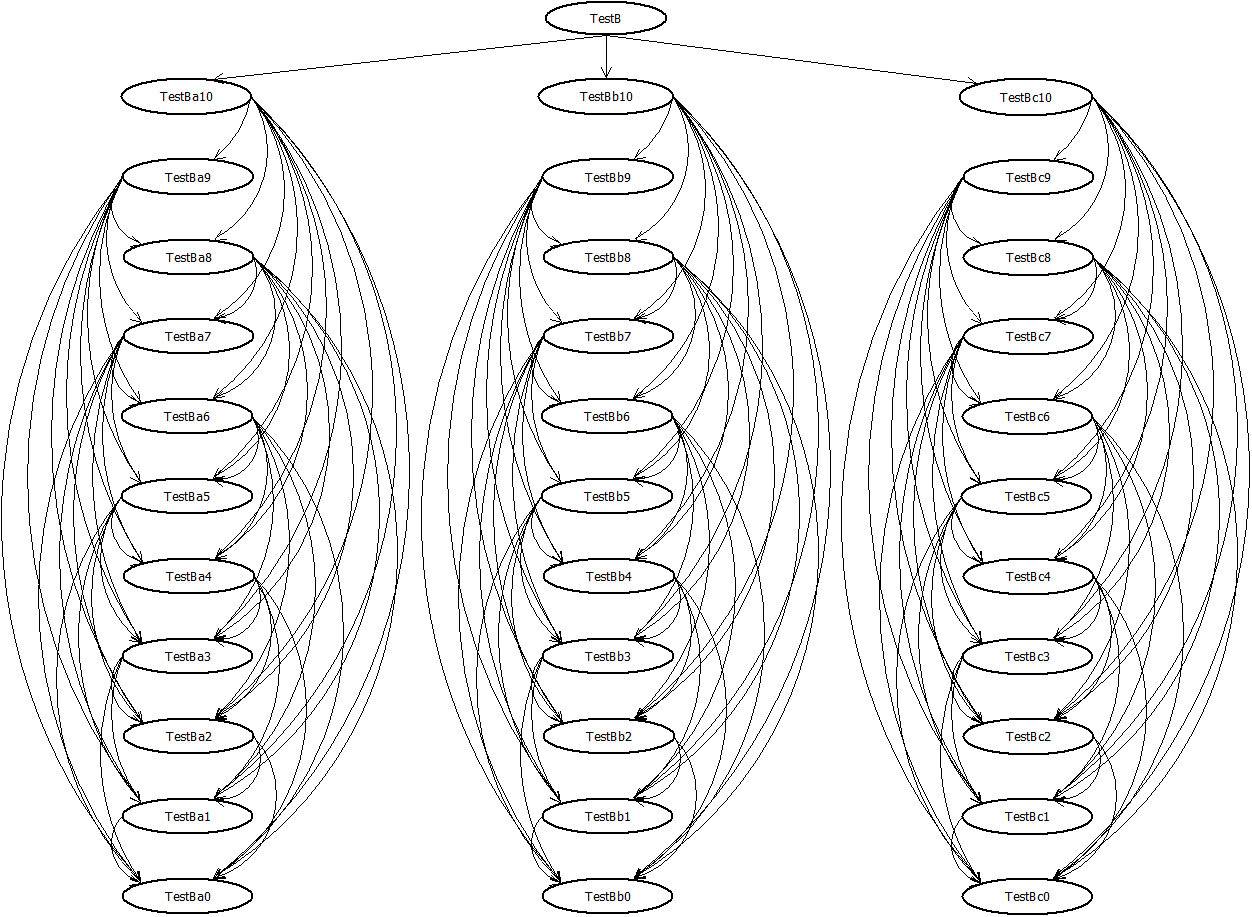
\includegraphics[width=\linewidth]{TestB.png}
  		\caption{Graf zależności dla testu B.}
  		\label{fig:testB}
	\end{center}
\end{figure}

Łatwo wywnioskować, że tworząc obiekty poszczególnych typów ilość tworzonych obiektów rośnie dwukrotnie (tak jak dla testu A):
\begin{itemize}
	\item TestBa0 - 1 obiekt,
	\item TestBa1 - 2 obiekty (obiekt typu TestBa1 i obiekt typu TestBa0),
	\item TestBa2 - 4 obiekty (obiekt typu TestBa2, obiekt typu TestBa1 - 2 obiekty, obiekt typu TestBa0 - 1 obiekt),
	\item TestBa3 - 8 obiektów (obiekt typu TestBa3, obiekt typu TestBa2 - 4 obiekty, obiekt typu TestBa1 - 2 obiekty, obiekt typu TestBa0 - 1 obiekt),
	\item TestBa4 - 16 obiektów,
	\item TestBa5 - 32 obiektów,
	\item TestBa6 - 64 obiektów,
	\item TestBa7 - 128 obiektów,
	\item TestBa8 - 256 obiektów,
	\item TestBa9 - 512 obiektów,
	\item TestBa10 - 1 024 obiektów,
	\item \ldots (dla typów od TestBb0 do TestBb10 i od TestBc0 do TestBc10 sytuacja wygląda dokłądnie tak samo jak dla typów od TestBa0 do TestBa10),
	\item TestB - 3 073 obiektów.
\end{itemize}
Zatem tworząc obiekt typu TestB, tworzymy: 1 obiekt typu TestB, 1 obiekt typu TestBa10, TestBb10 i TestBc10, 1 obiekt typu TestBa9, TestBb9 i TestBc9, 2 obiekty typu TestBa8, TestBb8 i TestBc8, 4 obiekty typu TestBa7, TestBb7 i TestBc7, 8 obiektów typu TestBa6, TestBb6 i TestBc6, 16 obiektów typu TestBa5, TestBb5 i TestBc5, 32 obiektów typu TestBa4, TestBb4 i TestBc4, 64 obiektów typu TestBa3, TestBb3 i TestBc3, 128 obiektów typu TestBa2, TestBb2 i TestBc2, 256 obiektów typu TestBa1, TestBb1 i TestBc1, 512 obiektów typu TestBa0, TestBb0 i TestBc0 - co daje w sumie 3 073 obiektów.

\subsubsection{Wyniki dla Register}
\begin{table}[H]
\captionsetup{belowskip=0pt,aboveskip=0pt}
\begin{center}
\begin{small}
	\begin{tabular}{ | l | r | r | r | r | }
    		\hline
Test & Singleton & Transient & TransientSingleton & PerThread \\ \hline
Autofac & 0 & 0 & 0 & 0 \\ \hline
DryIoc & 0 & 0 & 0 & 0 \\ \hline
Grace & 0 & 0 & 0 & 0 \\ \hline
LightInject & 0 & 0 & 0 & 0 \\ \hline
Ninject & 0 & 0 & 0 & 0 \\ \hline
NiquIoCPartial & 0 & 0 & 0 & 0 \\ \hline
NiquIoCFull & 0 & 0 & 0 & 0 \\ \hline
SimpleInjector & 0 & 0 & 0 & 0 \\ \hline
StructureMap & 1 & 1 & 1 & 1 \\ \hline
Unity & 0 & 0 & 0 & 0 \\ \hline
Windsor & 1 & 1 & 1 & 1 \\ \hline
  	\end{tabular}
\end{small}
\end{center}
\caption{Wyniki testów dla operacji Register dla Przypadku testowego B}
\label{TestCaseB_Register}
\end{table}
Tutaj wszystkie rozwiązania za wyjątkiem StructureMap i Windsor mają zawsze czasy zbliżone do 0. Te dwa rozwiązania wszystkich testów mają czasy zbliżone do 1 ms.

\subsubsection{Wyniki dla Singleton}
\begin{table}[H]
\captionsetup{belowskip=0pt,aboveskip=0pt}
\begin{center}
\begin{small}
	\begin{tabular}{ | l | r r r | r r r | r r r | r r r | }
    		\hline
Ilość & & 1 & & & 10 & & & 100 & & & 1000 & \\ \hline
 & min & max & avg & min & max & avg & min & max & avg & min & max & avg \\ \hline
Autofac & 0 & 0 & 0 & 0 & 0 & 0 & 0 & 0 & 0 & 0 & 0 & 0 \\ \hline
DryIoc & 8 & 8 & 8 & 8 & 9 & 8 & 8 & 9 & 8 & 8 & 9 & 8 \\ \hline
Grace & 8 & 8 & 8 & 8 & 8 & 8 & 8 & 8 & 8 & 8 & 8 & 8 \\ \hline
LightInject & 6 & 7 & 6 & 6 & 7 & 6 & 6 & 7 & 6 & 6 & 7 & 6 \\ \hline
Ninject & 9 & 10 & 9 & 9 & 10 & 9 & 9 & 11 & 10 & 12 & 13 & 12 \\ \hline
NiquIoCPartial & 4 & 4 & 4 & 4 & 4 & 4 & 4 & 5 & 4 & 4 & 4 & 4 \\ \hline
NiquIoCFull & 8 & 9 & 8 & 8 & 8 & 8 & 8 & 8 & 8 & 8 & 8 & 8 \\ \hline
SimpleInjector & 6 & 6 & 6 & 6 & 6 & 6 & 6 & 6 & 6 & 6 & 6 & 6 \\ \hline
StructureMap & 32 & 33 & 33 & 32 & 33 & 33 & 32 & 34 & 33 & 33 & 34 & 33 \\ \hline
Unity & 23 & 24 & 23 & 23 & 24 & 23 & 23 & 24 & 24 & 24 & 25 & 24 \\ \hline
Windsor & 0 & 0 & 0 & 0 & 0 & 0 & 0 & 0 & 0 & 0 & 0 & 0 \\ \hline
  	\end{tabular}
\end{small}
\end{center}
\caption{Wyniki testów dla operacji Singleton dla Przypadku testowego B}
\label{TestCaseB_Singleton}
\end{table}

Podobnie jak dla przypadku testowego A, tutaj również najlepiej poradziły sobie najpopularniejsze rozwiązania - Aurofac i Windsor. Warto zaznaczyć, że to jedyne rozwiązania, które nie zanotowały znaczącego wzrotu czasu. Dla pozostałych rozwiązań czasy wzrosły od 2 do 4 razy. NiquIoCPartial uplasował się tutaj również na 3 miejscu, a za nim SimpleInjector oraz LightInject. Koniec rankingu jest taki sam, czyli Ninject, Unity i StructureMap. NiquIoCFull, Grace, a także DryIoc miały zbliżone do siebie czasy - trochę słabsze niż LightInject i trochę lepsze niż Ninject.

\subsubsection{Wyniki dla Transient}
\begin{table}[H]
\captionsetup{belowskip=0pt,aboveskip=0pt}
\begin{center}
\begin{small}
	\begin{tabular}{ | l | r r r | r r r | r r r | r r r | }
    		\hline
Ilość & & 1 & & & 10 & & & 100 & & & 1000 & \\ \hline
 & min & max & avg & min & max & avg & min & max & avg & min & max & avg \\ \hline
Autofac & 2 & 2 & 2 & 21 & 25 & 21 & 189 & 201 & 191 & 1890 & 2044 & 1903 \\ \hline
DryIoc & 43 & 44 & 43 & 44 & 45 & 44 & 51 & 52 & 51 & 97 & 100 & 98 \\ \hline
Grace & 50 & 59 & 51 & 51 & 55 & 52 & 57 & 59 & 58 & 122 & 128 & 124 \\ \hline
LightInject & 31 & 33 & 32 & 32 & 33 & 32 & 37 & 38 & 37 & 70 & 73 & 71 \\ \hline
Ninject & 36 & 38 & 36 & 276 & 337 & 284 & 2733 & 3595 & 2790 & 28220 & 29976 & 28720 \\ \hline
NiquIoCPartial & 5 & 5 & 5 & 10 & 10 & 10 & 59 & 79 & 61 & 543 & 633 & 550 \\ \hline
NiquIoCFull & 26 & 27 & 26 & 26 & 27 & 26 & 32 & 33 & 32 & 66 & 68 & 66 \\ \hline
SimpleInjector & 40 & 41 & 40 & 40 & 42 & 41 & 47 & 48 & 47 & 95 & 97 & 96 \\ \hline
StructureMap & 33 & 34 & 33 & 45 & 46 & 45 & 167 & 175 & 168 & 1333 & 1565 & 1346 \\ \hline
Unity & 28 & 29 & 28 & 49 & 50 & 49 & 260 & 271 & 262 & 2355 & 2419 & 2366 \\ \hline
Windsor & 6 & 7 & 6 & 49 & 69 & 50 & 476 & 610 & 484 & 4726 & 5665 & 4799 \\ \hline
  	\end{tabular}
\end{small}
\end{center}
\caption{Wyniki testów dla operacji Transient dla Przypadku testowego B}
\label{TestCaseB_Transient}
\end{table}

Dla tego testu sytuacja wygląda niemal identycznie jak w teście A, z tą różnicą, że czasy dla każdego rozwiązania są ponad 3 razy większe.\\
Przy 1 operację najlepiej radzi sobie Autofac, a tuż za nim NiquIoCPartial i Windsor. Pozostałe rozwiązania wypadły słabo i mają czasy od kilku do kilkunastu razy większe niż czołówka. Kolejne miejsca to: NiquIocFull, Unity, LightInject, StructureMap oraz Ninject, a ranking zamykają SimplyInjector, DryIoc i Grace.\\
Gdy mamy 10 operacji najlepiej radzi sobie NiquIoCPartial, a zaraz za nim z czasem dwókrotnie gorszym jest Autofac. Następnie w rankingu znajduje się NiquIoCFull i LightInject. Tutaj również jak w przypadku testowym A, Ninject ma ponad 5 razy gorszy czas niż miejsce przedostatnie, z tą różnicą, że zajmuje je Grace, a nie Windsor, który uzyskał trochę lepszy czas i jest miejsce wyżej. Lepiej od Windsor poradziły sobie jeszcze: SimpleInjector, DryIoc, StructureMap i Unity, ale do czołówki brakowało im bardzo dużo.\\
Dla 100 operacji nic się nie zmieniło w stosunku do testu A. Pierwsze trzy miejsca zajmują: NiquIoCFull, LightInject i SimpleInjector. Grace z miejsca przedostatniego dla 10 operacji, awansował na miejsce piąte. Przed nim znalazł się DryIoc, a tuż za nim NiquIoCPartial. Czas całej trójki są zadowalające. Grono najsłabszych to: StructureMap, Autofac, Unity, Windsor i Ninject.\\
Jak można się było spodziewać przy 1000 operacji sytuacja wygląda identycznie - pod względem czasu od czołówki oddalił się NiquIoCPartial, a na pierwszym miejscu wciąż pozostaje NiquIoCFull. LightInject oraz SimpleInjector są kawałek za nim. Dalej DryIoc i Grace wciąż akceptowalnie. Miejsce w środku rankingu zajmuje NiquIoCPartial, a pozostałe rozwiązania mają od niego o rząd lub dwa większe czasy.\\
Tutaj również najmniejszy wzorst czasów miały rozwiązania: LightInject, NiquIoCFull, SimpleInjector, DryIoc oraz Grace.

\subsubsection{Wyniki dla TransientSingleton}
\begin{table}[H]
\captionsetup{belowskip=0pt,aboveskip=0pt}
\begin{center}
\begin{small}
	\begin{tabular}{ | l | r r r | r r r | r r r | r r r | }
    		\hline
Ilość & & 1 & & & 10 & & & 100 & & & 1000 & \\ \hline
 & min & max & avg & min & max & avg & min & max & avg & min & max & avg \\ \hline
Autofac & 1 & 2 & 1 & 18 & 20 & 18 & 172 & 206 & 173 & 1698 & 1832 & 1709 \\ \hline
DryIoc & 56 & 57 & 56 & 57 & 58 & 57 & 64 & 65 & 64 & 108 & 110 & 109 \\ \hline
Grace & 30 & 32 & 31 & 31 & 32 & 31 & 35 & 37 & 35 & 69 & 72 & 69 \\ \hline
LightInject & 48 & 50 & 48 & 48 & 50 & 48 & 51 & 53 & 51 & 80 & 82 & 80 \\ \hline
Ninject & 29 & 34 & 30 & 214 & 239 & 219 & 2013 & 2426 & 2063 & 20440 & 22891 & 20858 \\ \hline
NiquIoCPartial & 4 & 5 & 5 & 8 & 9 & 8 & 41 & 57 & 42 & 365 & 406 & 368 \\ \hline
NiquIoCFull & 16 & 16 & 16 & 16 & 17 & 16 & 18 & 19 & 18 & 37 & 39 & 38 \\ \hline
SimpleInjector & 28 & 28 & 28 & 28 & 29 & 28 & 32 & 34 & 32 & 61 & 62 & 61 \\ \hline
StructureMap & 33 & 34 & 33 & 40 & 46 & 40 & 112 & 123 & 113 & 797 & 915 & 805 \\ \hline
Unity & 27 & 28 & 27 & 46 & 47 & 46 & 226 & 263 & 228 & 2016 & 2305 & 2032 \\ \hline
Windsor & 3 & 5 & 3 & 37 & 46 & 37 & 355 & 435 & 362 & 3543 & 4824 & 3637 \\ \hline
  	\end{tabular}
\end{small}
\end{center}
\caption{Wyniki testów dla operacji TransientSingleton dla Przypadku testowego B}
\label{TestCaseB_TransientSingleton}
\end{table}
Jeśli chodzi o wzrost czasów w stosnku do przypadku testowego A, to sytuacja wygląda niemal identycznie jak dla testu Transient - jest on ponad trzykrotny.\\
Dla 1 operacji podium wygląda jednak inaczej niż dla testu A - miejscami zamieniły się NiquIocPartial i Windsor. Na pierwszy miejscu pozostaje Autofac. Różnice czasów dla pozostałych rozwiązań są już dużo bardziej zauważalne. Znajdujący się tuż za podium NiquIoCFull ma wynik ponad trzy razy słabszy niż NiquIoCPartial, który to podium zamyka. Kolejne miejsca to: Unity, SimpleInjector, Ninject, Grace, StructureMap, Lightinject i na końcu DryIoc.\\
Gry mamy 10 operacji pierwsze dwa miejsca zajmują NiquIoCPartial i NiquIoCFull. Tuż za nimi znajduje się Autofac. SimplyInjector oraz Grace zanotowały niewielki wzrost czasów i zajmują kolejne dwa miejsca. Nieduży wzrostu czasów zaliczyły również LightInject i DryIoc, ale ich czasy są wciąż duże w stosunku do pozostałych rozwiążań i zajmuje dwa przedostatnie miejsca - ustępując jedynie Ninject. Miejsca od 6 do 8 przypadły: Windsor, StructureMap oraz Unity.\\
Przy 100 i 1000 operacjach nie ma już żadnych zmian w rankingu względem testu A.\\
Dla pierwszego przypadku (100 operacji) początek rankingu wygląda następująco: NiquIocFull, SimpleInjector i Grace. Zaraz za podium znajduje się NiquIocPartial. LightInject oraz DryIoc dzięki niedużemu wzrostowi czasów znalazły się na miejscach piątym i szóstym. Są to ostatnie zadowalające rozwiązania. Kolejne miejsca zajmują: StrucutreMap, Autofac, Unity, Windsor oraz Ninject.\\
Dla drugiego przypadku (1000 operacji) pierwsze trzy miejsca są jak wyżej. Natomiast o jedno miejsce awansowały LightInject oraz Grace. NiquIoCPartial spadł na miejsce szóste i dołączył do grupy rozwiązań z bardzo dużymi czasami. Reszta rankingu nie uległa zmianie.

\subsubsection{Wyniki dla PerThread}
\begin{table}[H]
\captionsetup{belowskip=0pt,aboveskip=0pt}
\begin{center}
\begin{small}
	\begin{tabular}{ | l | r r r | r r r | r r r | r r r | }
    		\hline
Ilość & & 1 & & & 10 & & & 100 & & & 1000 & \\ \hline
 & min & max & avg & min & max & avg & min & max & avg & min & max & avg \\ \hline
Autofac & 0 & 0 & 0 & 0 & 0 & 0 & 0 & 0 & 0 & 0 & 0 & 0 \\ \hline
DryIoc & 246 & 250 & 247 & 246 & 250 & 247 & 246 & 248 & 247 & 246 & 249 & 247 \\ \hline
Grace & 13 & 13 & 13 & 13 & 13 & 13 & 13 & 14 & 13 & 13 & 14 & 13 \\ \hline
LightInject & 409 & 419 & 412 & 409 & 432 & 413 & 409 & 416 & 412 & 409 & 420 & 413 \\ \hline
Ninject & 9 & 10 & 9 & 9 & 10 & 9 & 9 & 10 & 10 & 12 & 13 & 13 \\ \hline
NiquIoCPartial & 4 & 5 & 4 & 4 & 4 & 4 & 4 & 4 & 4 & 4 & 5 & 4 \\ \hline
NiquIoCFull & 8 & 8 & 8 & 8 & 8 & 8 & 8 & 8 & 8 & 8 & 8 & 8 \\ \hline
SimpleInjector & 23 & 23 & 23 & 23 & 23 & 23 & 23 & 23 & 23 & 23 & 24 & 23 \\ \hline
StructureMap & 32 & 34 & 33 & 32 & 38 & 33 & 33 & 35 & 33 & 33 & 34 & 33 \\ \hline
Unity & 23 & 25 & 23 & 23 & 24 & 23 & 23 & 24 & 23 & 24 & 25 & 24 \\ \hline
Windsor & 0 & 0 & 0 & 0 & 0 & 0 & 0 & 0 & 0 & 0 & 0 & 0 \\ \hline
  	\end{tabular}
\end{small}
\end{center}
\caption{Wyniki testów dla operacji PerThread dla Przypadku testowego B}
\label{TestCaseB_PerThread}
\end{table}
Podobnie jak było dla przypadku testowego A, tutaj również nie wszystkie rozwiązania mają czasy zbliżone do Singleton.\\
Są to te same rozwiązania co dla testu A, czyli: SimpleInjector, DryIoc i LightInject. Warto jednak zaznaczyć, że dla SimpleInjector wzrost czasów jest kilkukrotny, a dla pozostałych dwóch rozwiązań kilkudziesięciokrotny.\\
Tak samo jak w przypadku Signleton czołówka wygląda następująco: Aurofac, Windsor i NiquIoCPartial. Kolejne miejsca zajmują: NiquIoCFull, Ninject i Grace. Najsłabiej poradziły sobie rozwiążania LightInject i DryIoc. W środku tabeli pod względem czasów znalazły się SimpleInjector, Unity i StrucutreMap. W odróżnieniu od przypadku testowego A, tutaj nie było żadnych zmian w rankingu i wszystkie rozwiązania zajmują te same miejsca dla dowolnej liczby operacji.

\subsubsection{Wyniki dla FactoryMethod}
\begin{table}[H]
\captionsetup{belowskip=0pt,aboveskip=0pt}
\begin{center}
\begin{small}
	\begin{tabular}{ | l | r r r | r r r | r r r | r r r | }
    		\hline
Ilość & & 1 & & & 10 & & & 100 & & & 1000 & \\ \hline
 & min & max & avg & min & max & avg & min & max & avg & min & max & avg \\ \hline
Autofac & 1 & 1 & 1 & 16 & 17 & 16 & 154 & 156 & 155 & 1545 & 1573 & 1550 \\ \hline
DryIoc & 0 & 0 & 0 & 1 & 2 & 1 & 19 & 19 & 19 & 185 & 188 & 186 \\ \hline
Grace & 7 & 9 & 7 & 10 & 10 & 10 & 38 & 39 & 39 & 312 & 319 & 315 \\ \hline
LightInject & 2 & 4 & 2 & 4 & 4 & 4 & 21 & 22 & 21 & 180 & 186 & 182 \\ \hline
Ninject & 23 & 25 & 24 & 166 & 182 & 170 & 1601 & 1670 & 1622 & 16788 & 17602 & 16963 \\ \hline
NiquIoCPartial & 0 & 0 & 0 & 4 & 4 & 4 & 37 & 39 & 38 & 364 & 373 & 368 \\ \hline
NiquIoCFull & 0 & 0 & 0 & 3 & 4 & 3 & 35 & 37 & 35 & 344 & 373 & 353 \\ \hline
SimpleInjector & 4 & 4 & 4 & 7 & 7 & 7 & 35 & 37 & 36 & 305 & 311 & 308 \\ \hline
StructureMap & 25 & 25 & 25 & 37 & 37 & 37 & 159 & 162 & 160 & 1347 & 1385 & 1359 \\ \hline
Unity & 4 & 6 & 4 & 44 & 45 & 44 & 436 & 443 & 439 & 4355 & 4492 & 4373 \\ \hline
Windsor & 4 & 5 & 4 & 33 & 36 & 33 & 298 & 321 & 301 & 2939 & 3226 & 2971 \\ \hline
  	\end{tabular}
\end{small}
\end{center}
\caption{Wyniki testów dla operacji FactoryMethod dla Przypadku testowego B}
\label{TestCaseB_FactoryMethod}
\end{table}
Tym razem dla 1 operacji czas poniżej 1 ms osiągnęły: DryIoc, NiquIoCPartial i NiquIoCFull. Zaraz za nimi znalazł się Autofac. Kawałek dalej LightInject, a następnie SimpleInjector, Windsor i Unity. Dziewiąte miejsce zajął Grace i miał on czas około dwa razy gorszy od ósmego Unity. Dwa ostatnie miejsca przypadły StructureMap i Ninject, które osiągnęły zbliżone czasy, ale ponad 3 razy większe niż Grace.\\
Przy 10 operacjach pierwsze trzy miejsca się nie zminieły, czyli: DryIoc, NiquIoCFull i NiquIoCParial. Jednakże tym razem różnice czasu między nimi zaczynają być lekko dostrzegalne. Czasy zbliżone do czołówki do miał również LightInject. Kolejne dwa miejsca przypadły SimpljeInjector oraz Grace. Podobnie jak dla przypadku testowego A, tym razem również na siódme miejsce spadł Autofac. Pozostałe rozwiązania osiągnęły czasy conajmniej dwukrotnie większe od niego i są to kolejno: Windsor, StructureMap, Unity i na końcu Ninject z czasem około czterokrotnie większym niż przedostatni Unity.\\
Gdy mamy 100 operacji czołówka uległa roszadom i wdarł się do niej SimpleInjector oraz Grace. Tym razem pierwsza połowa rankingu to na początku DryIoc oraz LightInject, a kawałek za nimi NiquIoCFull, SimpleInjector,  NiquIoCPartial i Grace. Na następnych dwóch pozycjach znalazły się AutoFac i StructureMap z czasami zbliżonymi do siebie, ale około czterokrotnie większymi niż czołówka. Na miejsce dziewiąte spadł Windsor, a ostatnie dwa zajmęły Unity i Ninject.\\
Dla 1000 operacji NiquIoCFull spadł na piąte miejsce. Przed nim znalazły się kolejno: DryIoc i LightInject. ze sporą przewagą nad resztą, a dalej SimpleInjector oraz Grace. Kawałek za nim znalazł się NiquIoCPartial. Drugą połowę ranking otwiera StructureMap, który poradził sobie trochę lepiej niż Autofac. Oba te rozwiązania mają czasy ponad trzy razy większe niż pierwsza szóstka, ale również około dwa razy mniejsze niż ostatnia trójka. Ranking zamykają: Windsor, Unity i Ninject.


\subsection{Przypadek testowy C}
\subsubsection{Opis}
Ten przypadek testowy znacząco różni się od dwóch poprzednich. Mamy tutaj zdefiniowanych 26 typów. 5 z tych typów ma konstruktor bezparametrowy, a pozostałe 21 ma konstuktor z pięcioma parametrami. Typem głównym jest typ "TestC". Obiekt tego typy w konstruktorze przymuje 5 obiektów, kolejno następujących typów: "TestC40", "TestC41", "TestC42", "TestC43" i "TestC44". Każdy z tych pięciu typów ma taki sam konstruktor - przyjmuje w nim 5 obiektów o typach, które w nazwie mają pierwszy numer o 1 mniejszy, czyli są to obiekty typów od "TestC30" do "TestC34". Dla tych i kolejnych typów zasad z konstruktorami wygląda tak samo. Na końcu dochodzimy do typów od "TestC00" do "TestC04", które mają konstruktor bezparametrowy. Rys. \ref{fig:testC} przedstawia graf zależności typów dla tego przypadku testowego.\\
\begin{figure}[H]
	\begin{center}
  		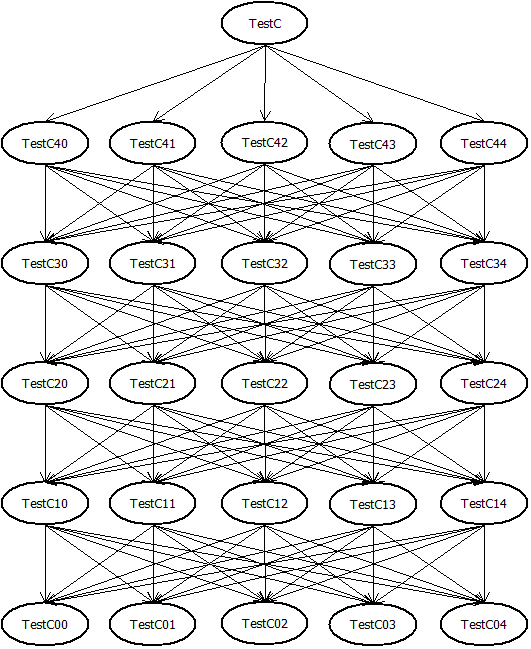
\includegraphics[height=11.5cm]{TestC.png}
  		\caption{Graf zależności dla testu C.}
  		\label{fig:testC}
	\end{center}
\end{figure}

Łatwo wywnioskować, że tworząc obiekty poszczególnych typów ilość tworzonych obiektów rośnie ponad pięciokrotnie:
\begin{itemize}
	\item typy od TestC00 do TestC04 - 1 obiekt,
	\item typy od TestC10 do TestC14 - 6 obiektów (obiekt danego typu plus 5 obiektów typów od TestC00 do TestC04),
	\item typy od TestC20 do TestC24 - 31 obiektów (obiekt danego typu plus 5 obiektów typów od TestC10 do TestC14),
	\item typy od TestC30 do TestC34 - 156 obiektów,
	\item  typy od TestC40 do TestC44 - 781 obiektów,
	\item TestC - 3 906 obiektów.
\end{itemize}
Zatem tworząc obiekt typu TestC, tworzymy: 1 obiekt typu TestC, 5 obiektów typów od TestC40 do TestC44, 25 obiektów typów od TestC30 do TestC34, 125 obiektów typów od TestC20 do TestC24, 625 obiektów typów od TestC10 do TestC14 oraz 3 125 obiektów typów od TestC00 do TestC04 - co daje w sumie 3 906 obiektów.

\subsubsection{Wyniki dla Register}
\begin{table}[H]
\captionsetup{belowskip=0pt,aboveskip=0pt}
\begin{center}
\begin{small}
	\begin{tabular}{ | l | r | r | r | r | }
    		\hline
Test & Singleton & Transient & TransientSingleton & PerThread \\ \hline
Autofac & 0 & 0 & 0 & 0 \\ \hline
DryIoc & 0 & 0 & 0 & 0 \\ \hline
Grace & 0 & 0 & 0 & 0 \\ \hline
LightInject & 0 & 0 & 1 & 0 \\ \hline
Ninject & 0 & 0 & 0 & 0 \\ \hline
NiquIoCPartial & 0 & 0 & 0 & 0 \\ \hline
NiquIoCFull & 0 & 0 & 0 & 0 \\ \hline
SimpleInjector & 0 & 0 & 0 & 0 \\ \hline
StructureMap & 1 & 1 & 1 & 1 \\ \hline
Unity & 0 & 0 & 0 & 0 \\ \hline
Windsor & 0 & 0 & 0 & 0 \\ \hline
  	\end{tabular}
\end{small}
\end{center}
\caption{Wyniki testów dla operacji Register dla Przypadku testowego C}
\label{TestCaseC_Register}
\end{table}
Tym razem wszystkie rozwiązania za wyjątkiem LightInject i StructureMap mają zawsze czasy zbliżone do 0. LightInject dla testu TransientSingleton ma czas zbliżony do 1 ms, a StructureMap dla wszystkich testów.

\subsubsection{Wyniki dla Singleton}
\begin{table}[H]
\captionsetup{belowskip=0pt,aboveskip=0pt}
\begin{center}
\begin{small}
	\begin{tabular}{ | l | r r r | r r r | r r r | r r r | }
    		\hline
Ilość & & 1 & & & 10 & & & 100 & & & 1000 & \\ \hline
 & min & max & avg & min & max & avg & min & max & avg & min & max & avg \\ \hline
Autofac & 0 & 0 & 0 & 0 & 0 & 0 & 0 & 0 & 0 & 0 & 0 & 0 \\ \hline
DryIoc & 5 & 5 & 5 & 5 & 5 & 5 & 5 & 5 & 5 & 5 & 5 & 5 \\ \hline
Grace & 5 & 5 & 5 & 5 & 5 & 5 & 5 & 5 & 5 & 5 & 5 & 5 \\ \hline
LightInject & 4 & 4 & 4 & 4 & 4 & 4 & 4 & 4 & 4 & 4 & 4 & 4 \\ \hline
Ninject & 6 & 6 & 6 & 6 & 6 & 6 & 6 & 7 & 6 & 9 & 10 & 9 \\ \hline
NiquIoCPartial & 3 & 3 & 3 & 3 & 3 & 3 & 3 & 3 & 3 & 3 & 3 & 3 \\ \hline
NiquIoCFull & 5 & 5 & 5 & 5 & 5 & 5 & 5 & 5 & 5 & 5 & 5 & 5 \\ \hline
SimpleInjector & 4 & 4 & 4 & 4 & 4 & 4 & 4 & 4 & 4 & 4 & 4 & 4 \\ \hline
StructureMap & 22 & 23 & 22 & 22 & 23 & 22 & 22 & 23 & 22 & 23 & 24 & 23 \\ \hline
Unity & 15 & 16 & 15 & 15 & 16 & 15 & 15 & 16 & 15 & 16 & 17 & 16 \\ \hline
Windsor & 0 & 0 & 0 & 0 & 0 & 0 & 0 & 0 & 0 & 0 & 0 & 0 \\ \hline
  	\end{tabular}
\end{small}
\end{center}
\caption{Wyniki testów dla operacji Singleton dla Przypadku testowego C}
\label{TestCaseC_Singleton}
\end{table}
Pomimo zupełnie innego przypadku testowego, dla testu Singleton, wciąż najlepiej radzą sobie Autofac i Windsor. Ich czasy nawet dla 1000 operacji są wciąż mniejsze niż 1 milisekunda. Dodatkowo tutaj również podium zamyka NiquIoCPartial. Kolejne miejsca zajmują LightInject i SimpleInjector. Trochę gorzej od nich radzą sobie DryIoc, Grace i NiquIoCFull. Ostatnie trzy miejsca należą do Ninject, Unity i StructureMap. Zatem ranking wygląda tutaj identycznie jak dla poprzednich dwóch testów dla tego samego przypadku.

\subsubsection{Wyniki dla Transient}
\begin{table}[H]
\captionsetup{belowskip=0pt,aboveskip=0pt}
\begin{center}
\begin{small}
	\begin{tabular}{ | l | r r r | r r r | r r r | r r r | }
    		\hline
Ilość & & 1 & & & 10 & & & 100 & & & 1000 & \\ \hline
 & min & max & avg & min & max & avg & min & max & avg & min & max & avg \\ \hline
Autofac & 2 & 2 & 2 & 23 & 25 & 24 & 229 & 250 & 231 & 2274 & 2419 & 2288 \\ \hline
DryIoc & 39 & 41 & 39 & 40 & 41 & 40 & 47 & 48 & 47 & 98 & 100 & 99 \\ \hline
Grace & 61 & 63 & 61 & 62 & 65 & 62 & 73 & 74 & 73 & 153 & 163 & 155 \\ \hline
LightInject & 36 & 37 & 36 & 36 & 39 & 37 & 43 & 49 & 44 & 86 & 88 & 86 \\ \hline
Ninject & 38 & 42 & 39 & 345 & 375 & 353 & 3430 & 4043 & 3511 & 36072 & 42914 & 37642 \\ \hline
NiquIoCPartial & 3 & 4 & 4 & 10 & 11 & 10 & 72 & 80 & 74 & 683 & 781 & 690 \\ \hline
NiquIoCFull & 31 & 33 & 31 & 31 & 33 & 32 & 38 & 41 & 38 & 81 & 83 & 82 \\ \hline
SimpleInjector & 40 & 42 & 41 & 41 & 43 & 41 & 49 & 51 & 49 & 115 & 117 & 116 \\ \hline
StructureMap & 26 & 27 & 26 & 40 & 42 & 40 & 178 & 207 & 181 & 1520 & 1810 & 1540 \\ \hline
Unity & 18 & 19 & 19 & 47 & 51 & 47 & 315 & 369 & 318 & 2995 & 3359 & 3015 \\ \hline
Windsor & 7 & 8 & 7 & 61 & 82 & 62 & 594 & 769 & 608 & 5898 & 7708 & 6037 \\ \hline
  	\end{tabular}
\end{small}
\end{center}
\caption{Wyniki testów dla operacji Transient dla Przypadku testowego C}
\label{TestCaseC_Transient}
\end{table}
Gdy mamy 1 operację najniższe czasy uzyskały Autofac i NiquIoCPartial. Tuż za nimi znalazł się Windsor. Kolejne rozwiązania mają już dużo większe czasy. Na czwartym miejscu znalazł się Unity, dalej StructureMap i NiquIoCFull. Następne miejsca należą kolejno do LightInject, DryIoc, Ninject i SimpleInjector. Najgorzej poradził sobie tutaj Grace.\\
Przy 10 operacjach pierwsze dwa miejsca uległy zamianie. Tym razem najniższe czasy uzyskał NiquIoCPartial. Podium zamyka NiquIoCFull, który awansował o 3 miejsca. Niewiele za nim uplasował się LightInject. Kolejne pozycje w rankingu należą do DryIoc, StructureMap oraz SimpleInjector, które uzyskały zbliżone do siebie czasy. Znaczący wzrost czasów zanotowały natomiast Unity i Windsor, które znalazły się na miejsach 8 i 10. Z niewielkim wzrostem czasu w stosunku do 1 operacji, między nimi znalazł się Grace. Ranking zamyka Ninject.\\
Dla 100 operacji na prowadzenie wysunęły się NiquIoCFull oraz LightInject. Trochę słabiej poradziły sobie DryIoc i SimpleInjector, jednak ich czasy są również zadowalające. Następne miejsca z zauważalną różnicą czasów w stosunku do czołówki zajęły Grace oraz NiquIoCPartial. Miejsce 7 w rankingu zajął StructureMap z czasem ponad dwukrotnie większym niż poprzednik. Kolejne miejsca należą do: Autofac, Unity, Windsor i Ninject.\\
Test dla 1000 operacji nie spowodował żadnych zmian w rankingu, jednakże czasy dla NiquIoCPartial przestały być akceptowalne - wzrosły one ponad dziewięciokrotnie, a dla wyższych miejsc wzrost był maksymalnie trzykrotny. Pozostałe rozwiązania miały wzrost zbliżony do wzorstu NiquIoCPartial.

\subsubsection{Wyniki dla TransientSingleton}
\begin{table}[H]
\captionsetup{belowskip=0pt,aboveskip=0pt}
\begin{center}
\begin{small}
	\begin{tabular}{ | l | r r r | r r r | r r r | r r r | }
    		\hline
Ilość & & 1 & & & 10 & & & 100 & & & 1000 & \\ \hline
 & min & max & avg & min & max & avg & min & max & avg & min & max & avg \\ \hline
Autofac & 1 & 2 & 2 & 19 & 20 & 20 & 184 & 198 & 187 & 1810 & 1898 & 1831 \\ \hline
DryIoc & 58 & 70 & 58 & 59 & 62 & 59 & 65 & 68 & 65 & 105 & 107 & 106 \\ \hline
Grace & 23 & 24 & 23 & 23 & 24 & 23 & 25 & 26 & 25 & 44 & 45 & 44 \\ \hline
LightInject & 52 & 54 & 52 & 52 & 55 & 53 & 55 & 57 & 56 & 82 & 85 & 83 \\ \hline
Ninject & 25 & 30 & 26 & 199 & 231 & 203 & 1903 & 2364 & 1951 & 19137 & 22595 & 19626 \\ \hline
NiquIoCPartial & 3 & 3 & 3 & 6 & 7 & 6 & 38 & 46 & 39 & 347 & 359 & 349 \\ \hline
NiquIoCFull & 12 & 13 & 12 & 12 & 13 & 12 & 13 & 14 & 14 & 25 & 26 & 25 \\ \hline
SimpleInjector & 21 & 22 & 21 & 21 & 22 & 21 & 23 & 24 & 24 & 44 & 45 & 44 \\ \hline
StructureMap & 23 & 23 & 23 & 30 & 31 & 30 & 80 & 84 & 80 & 549 & 593 & 553 \\ \hline
Unity & 18 & 18 & 18 & 39 & 41 & 40 & 242 & 258 & 243 & 2258 & 2428 & 2272 \\ \hline
Windsor & 3 & 3 & 3 & 34 & 41 & 35 & 338 & 400 & 343 & 3368 & 4115 & 3429 \\ \hline
  	\end{tabular}
\end{small}
\end{center}
\caption{Wyniki testów dla operacji TransientSingleton dla Przypadku testowego C}
\label{TestCaseC_TransientSingleton}
\end{table}
Dla 1 operacji tylko 3 rozwiążania uzyskały wynik jednocyfrowy. Są to kolejno: Autofac, NiquIoCPartial i Windsor. Pozsotałe rozwiązania czasy mają dużo słabsze. Najniższy uzyskał NiquIoCPartial, a dalej za nim Unity i SimpleInjector. Kolejne miejsca należą do StrucutreMap, Grace i Ninject. Na końcu rankingu znalazły się LightInject oraz DryIoc.\\
Przy 10 operacjach sytuacja lekko uległą zmianie. Pierwsze dwa miejsca zajmują NiquIoCPartial i NiquIoCFull. Kawałek za nimi są Autofac i SimpleInjector, które dzieli niewielka różnica. Trochę gorszy czas od nich uzyskał Grace. Reszta rozwiązań dość znacząco odstaje od czołówki. Ostatnie 6 miejsc to: StructureMap, Windsor, Unity, LightInject, DryIoc oraz na końcu Ninject.\\
Gdy mamy 100 operacji na prowadzenie wysunął się NiquIoCFull, a poza pierwszą trójkę wypadł NiquIoCPartial. Miejsce drugie i trzecie należą do SimpleInjector oraz Grace. LightInject i DryIoc zanotowały niewielki wzrost czasów i przy dużym wzroście dla pozostałych rozwiązań, znalazły się na miejscach 5 i 6. Do grona najsłabszych dołączył natomiast Autofac. Zajął on miejsce pomiędzy StrucuteMap, a Unity. Ostatnia pozycja nie uległa zmianie i należy do Ninejct, przed którym znalazł się Windsor.\\
Również i dla tego testu przy 1000 operacjach nie było dużych zmian w rankingu. Wszystkie rozwiązania zachowały swoje miejsca za wyjątkiem NiquIoCPartial, który spadł na miejsce 6.

\subsubsection{Wyniki dla PerThread}
\begin{table}[H]
\captionsetup{belowskip=0pt,aboveskip=0pt}
\begin{center}
\begin{small}
	\begin{tabular}{ | l | r r r | r r r | r r r | r r r | }
    		\hline
Ilość & & 1 & & & 10 & & & 100 & & & 1000 & \\ \hline
 & min & max & avg & min & max & avg & min & max & avg & min & max & avg \\ \hline
Autofac & 0 & 0 & 0 & 0 & 0 & 0 & 0 & 0 & 0 & 0 & 0 & 0 \\ \hline
DryIoc & 157 & 162 & 158 & 157 & 160 & 158 & 157 & 160 & 158 & 158 & 161 & 158 \\ \hline
Grace & 8 & 9 & 8 & 8 & 9 & 8 & 8 & 9 & 8 & 8 & 9 & 8 \\ \hline
LightInject & 525 & 556 & 529 & 525 & 551 & 530 & 525 & 558 & 530 & 525 & 550 & 529 \\ \hline
Ninject & 6 & 7 & 6 & 6 & 6 & 6 & 6 & 7 & 6 & 9 & 10 & 9 \\ \hline
NiquIoCPartial & 3 & 3 & 3 & 3 & 3 & 3 & 3 & 3 & 3 & 3 & 3 & 3 \\ \hline
NiquIoCFull & 5 & 5 & 5 & 5 & 5 & 5 & 5 & 5 & 5 & 5 & 5 & 5 \\ \hline
SimpleInjector & 16 & 16 & 16 & 16 & 16 & 16 & 16 & 16 & 16 & 16 & 18 & 16 \\ \hline
StructureMap & 22 & 23 & 22 & 22 & 23 & 22 & 22 & 23 & 22 & 23 & 73 & 24 \\ \hline
Unity & 15 & 16 & 15 & 15 & 16 & 15 & 15 & 16 & 15 & 16 & 17 & 16 \\ \hline
Windsor & 0 & 0 & 0 & 0 & 0 & 0 & 0 & 0 & 0 & 0 & 0 & 0 \\ \hline
  	\end{tabular}
\end{small}
\end{center}
\caption{Wyniki testów dla operacji PerThread dla Przypadku testowego C}
\label{TestCaseC_PerThread}
\end{table}
Podobnie jak dla przypadków testowych A i B, tutaj również SimpleInjector zaliczył lekki wzrost czasów w stosunku do testu Singleton. DryIoc oraz LightInject zaliczyły bardzo duże wzrosty i to one zamykają ranking. Przed nimi znalazł się StructureMap, a miejsce wyżej wcześniej wspomniany SimpleInjector. Podobne czasy do niego zanotował Unity, który uplasował się na miejscu 7. Idąc w rankingu ku górze, to przy 1, 10 i 100 operacjach lepiej radził Ninject, a przy 1000 operacjach Grace. Te dwa rozwiązania znalazły się na dwóch kolejnych miejscach. Tuż za podium jest NiquIoCFull, a pierwsze trzy miejsca bez zmian dla tego testu, czyli: Autofac, Windsor, NiquIoCPartial.

\subsubsection{Wyniki dla FactoryMethod}
\begin{table}[H]
\captionsetup{belowskip=0pt,aboveskip=0pt}
\begin{center}
\begin{small}
	\begin{tabular}{ | l | r r r | r r r | r r r | r r r | }
    		\hline
Ilość & & 1 & & & 10 & & & 100 & & & 1000 & \\ \hline
 & min & max & avg & min & max & avg & min & max & avg & min & max & avg \\ \hline
Autofac & 2 & 2 & 2 & 19 & 21 & 19 & 186 & 197 & 189 & 1867 & 1979 & 1880 \\ \hline
DryIoc & 0 & 0 & 0 & 2 & 2 & 2 & 24 & 25 & 24 & 232 & 236 & 234 \\ \hline
Grace & 6 & 6 & 6 & 9 & 9 & 9 & 42 & 44 & 42 & 357 & 369 & 361 \\ \hline
LightInject & 2 & 2 & 2 & 4 & 5 & 4 & 24 & 27 & 25 & 215 & 223 & 218 \\ \hline
Ninject & 26 & 28 & 27 & 209 & 220 & 213 & 2110 & 2474 & 2152 & 22141 & 23030 & 22398 \\ \hline
NiquIoCPartial & 0 & 0 & 0 & 5 & 5 & 5 & 45 & 47 & 46 & 446 & 479 & 451 \\ \hline
NiquIoCFull & 0 & 0 & 0 & 4 & 4 & 4 & 42 & 45 & 43 & 419 & 440 & 424 \\ \hline
SimpleInjector & 3 & 4 & 3 & 7 & 7 & 7 & 43 & 45 & 44 & 380 & 389 & 385 \\ \hline
StructureMap & 18 & 20 & 18 & 34 & 35 & 34 & 177 & 198 & 180 & 1594 & 1748 & 1623 \\ \hline
Unity & 6 & 7 & 6 & 56 & 58 & 56 & 555 & 645 & 564 & 5561 & 5645 & 5577 \\ \hline
Windsor & 4 & 5 & 4 & 38 & 41 & 39 & 366 & 378 & 369 & 3650 & 4077 & 3721 \\ \hline
  	\end{tabular}
\end{small}
\end{center}
\caption{Wyniki testów dla operacji FactoryMethod dla Przypadku testowego C}
\label{TestCaseC_FactoryMethod}
\end{table}
Dla tego testu ranking również jest bardzo podobny, jak dla przypadków testowych A i B. Występują jedynie drobne rotacje na niektórych pozycjach, ale czasy są do siebie podobnie zbliżone.\\
Tak więc dla 1 operacji początek rankingu to: DryIoc, NiquIoCPartial i NiquIocFull. Za nimi znalazły się Autofac i LightInject. Na kolejnych pozycjach z niedużą stratą do czołówki są: SimpleInjector, Windsor, Grace oraz Unity. Przedostatnie miejsce zajął StructureMap, który ma czas około trzy razy gorszy niż Unity (znajdujący się miejsce wyżej) i prawie o połowę mniejszy niż ostatni Ninject.\\
Gdy mamy 10 operacjach pierwsza czwórka wygląda nastepująco: DryIoc, NiquIoCFull, LightInject oraz NiquIoCPartial. Kolejne dwa miejsca przypadły SimpljeInjector i Grace, ale ich czasy są zauważalnie większe niż rozwiązań z początku rankingu. Ponownie na miejsce siódme spadł Autofac z czasami ponad dwa razy słabszymi niż znajdujący niż na szóstym miejscu Grace, ale również z czasami prawie dwa razy lepszymi niż StructureMap, który znalazł się na miejscu ósmym. Trochę słabiej od StructureMap poradził sobie Windsor. Ranking zamykają Unity i Ninject.\\
Przy 100 operacji Grace wyprzedził NiquIoCFull, a SimpleInjector NiquIoCPartial. Pierwsza szóstka prezentuje się następująco: DryIoc oraz LightInject i kawałek za nimi Grace, NiquIoCFull, SimpleInjector oraz NiquIoCPartial. Autofac spadł o jedną pozycję, a wyprzedził go StructureMap. Ostatnie trzy miejsca bez zmian, a więc: Windsor, Unity oraz Ninject.\\
Dla 1000 operacji na pierwsze miejsce wskoczył LightInject, a na drugie spadł DryIoc. Kolejne miejsca z zauważalną stratą do pierwszej dwójki zajęły: Grace, SimpleInjector, NiquIoCFull i NiquIoCPartial. Druga połowa rankingu nie uległa już zmienie i na kolejnych pozycjach znalazły się: StructureMap, Autofac, Windsor, Unity oraz Ninject.


\subsection{Przypadek testowy D}
\subsubsection{Opis}
Podobnie jak przypadek testowy B jest analigoczny z przypadkiem A, tak ten przypadek, jest zbliżony do przypadku C. Jednakże pokrewieństwo jest inne. Mamy tutaj tyle sama poziomów, co dla C, ale na każdym poziomie (poza pierwszym) obiektów jest dwa razy więcej. Zatem w tym teście mamy zdefiniowanych 51 typów. Tutaj konstruktor bezparametrowy ma 10 typów, a pozostałe 41 ma konstuktor z dziesięcioma parametrami. Typ główny to "TestD" i przymuje on w konstruktorze 10 obiektów, kolejno następujących typów: "TestD40", "TestD41", "TestD42", "TestD43", "TestD44", "TestD45", "TestD46", "TestD47", "TestD48", "TestD49". Jest więc to sytuacja niemal identyczna jak dla poprzedniego przypadku. Dla pozostałych typów jest podobnie i każdy z nich w konstruktorze przyjmuje 10 obiektów o typach z pierwszym numerem o 1 mniejszym (obiekty typów od "TestD40" do "TestD49", przyjmują w konstruktorze obiekty typów od "TestD30" do "TestD39" itd.). Ostatnie 10 typów, czyli typy od "TestD00" do "TestD09", mają konstruktor bezparametrowy. Graf zależności dla tego przypadku testowego został przedstawiony na Rys. \ref{fig:testD}.\\
\begin{figure}[H]
	\begin{center}
  		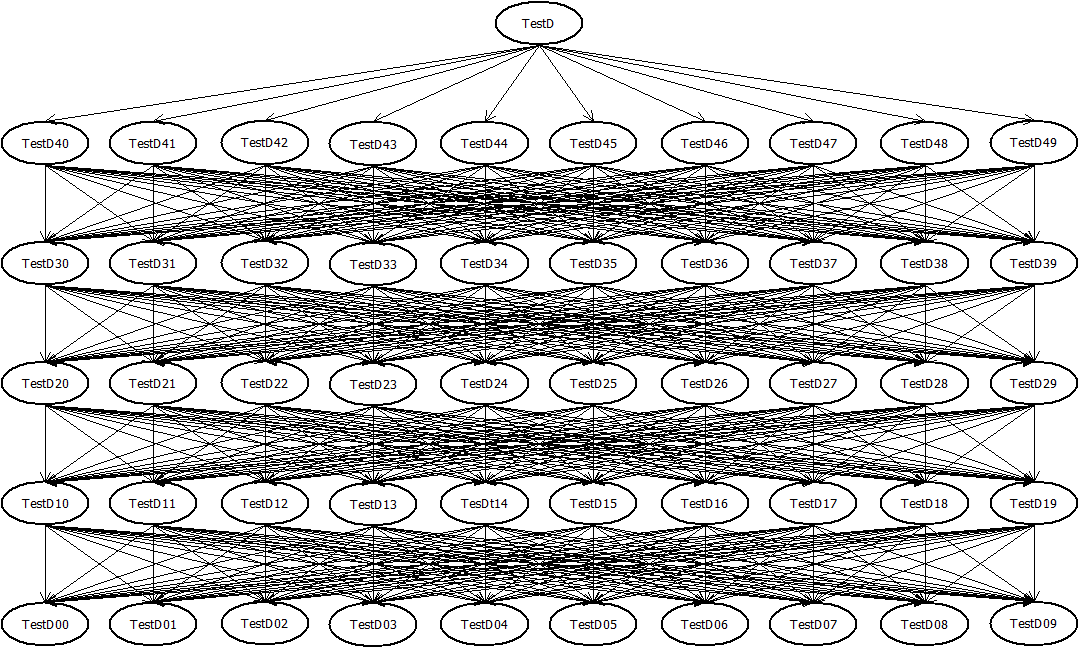
\includegraphics[width=\linewidth]{TestD.png}
  		\caption{Graf zależności dla testu D.}
  		\label{fig:testD}
	\end{center}
\end{figure}

Łatwo wywnioskować, że tworząc obiekty poszczególnych typów ilość tworzonych obiektów rośnie ponad dziesięciokortnie:
\begin{itemize}
	\item typy od TestD00 do TestD09 - 1 obiekt,
	\item typy od TestD10 do TestD19 - 11 obiektów (obiekt danego typu plus 10 obiektów typów od TestD00 do TestD09),
	\item typy od TestD20 do TestD29 - 111 obiektów (obiekt danego typu plus 10 obiektów typów od TestD10 do TestD19),
	\item typy od TestD30 do TestD39 - 1 111 obiektów,
	\item  typy od TestD40 do TestD49 - 11 111 obiektów,
	\item TestD - 111 111 obiektów.
\end{itemize}
Zatem tworząc obiekt typu TestD, tworzymy: 1 obiekt typu TestD, 10 obiektów typów od TestD40 do TestD49, 100 obiektów typów od TestD30 do TestD39, 1 000 obiektów typów od TestD20 do TestD29, 10 000 obiektów typów od TestD10 do TestD19, 100 000 obiektów typów od TestD00 do TestD09 - co daje w sumie 111 111 obiektów.

\subsubsection{Wyniki dla Register}
\begin{table}[H]
\captionsetup{belowskip=0pt,aboveskip=0pt}
\begin{center}
\begin{small}
	\begin{tabular}{ | l | r | r | r | r | }
    		\hline
Test & Singleton & Transient & TransientSingleton & PerThread \\ \hline
Autofac & 0 & 0 & 0 & 0 \\ \hline
DryIoc & 0 & 0 & 0 & 0 \\ \hline
Grace & 0 & 0 & 0 & 0 \\ \hline
LightInject & 0 & 0 & 0 & 0 \\ \hline
Ninject & 0 & 0 & 0 & 0 \\ \hline
NiquIoCPartial & 0 & 0 & 0 & 0 \\ \hline
NiquIoCFull & 0 & 0 & 0 & 0 \\ \hline
SimpleInjector & 0 & 0 & 0 & 0 \\ \hline
StructureMap & 4 & 2 & 1 & 4 \\ \hline
Unity & 0 & 0 & 0 & 0 \\ \hline
Windsor & 1 & 1 & 1 & 2 \\ \hline
  	\end{tabular}
\end{small}
\end{center}
\caption{Wyniki testów dla operacji Register dla Przypadku testowego D}
\label{TestCaseD_Register}
\end{table}
Dla tego przypadku testowego również wszystkie rozwiązania za wyjątkiem StructureMap i Windsor mają czasy zbliżone do 0 ms. StructureMap radzi sobie zdecydowanie najgorzej. Zarówno dla testu Singleton jak i PerThread osiągnął czas 4 ms. Dla Transient zanotował 2 ms, a dla TransientSingleton 1 ms. Windsor natomiast dla trzech pierwszych testów (Singleton, Transient oraz TransientSingleton) ma czas zbliżony do 1 ms, a dla ostatniego testu (PerThread) osiąga 2 ms.

\subsubsection{Wyniki dla Singleton}
\begin{table}[H]
\begin{center}
\begin{small}
	\begin{tabular}{ | l | r r r | r r r | }
    		\hline
Ilość & & 1 & & & 10 & \\ \hline
 & min & max & avg & min & max & avg \\ \hline
Autofac & 0 & 0 & 0 & 0 & 0 & 0 \\ \hline
DryIoc & 10 & 10 & 10 & 10 & 10 & 10 \\ \hline
Grace & 16 & 17 & 16 & 16 & 17 & 16 \\ \hline
LightInject & 14 & 14 & 14 & 14 & 15 & 14 \\ \hline
Ninject & 21 & 22 & 21 & 21 & 22 & 21 \\ \hline
NiquIoCPartial & 8 & 9 & 9 & 8 & 9 & 8 \\ \hline
NiquIoCFull & 18 & 19 & 18 & 18 & 19 & 18 \\ \hline
SimpleInjector & 11 & 12 & 11 & 11 & 12 & 11 \\ \hline
StructureMap & 49 & 50 & 49 & 49 & 50 & 49 \\ \hline
Unity & 52 & 53 & 52 & 52 & 54 & 52 \\ \hline
Windsor & 0 & 0 & 0 & 0 & 0 & 0 \\ \hline
  	\end{tabular}
\end{small}
\end{center}
\caption{Wyniki testów dla operacji Singleton dla Przypadku testowego D}
\label{TestCaseD_Singleton}
\end{table}
W porówaniu do poprzednich przypadków testowych, różnice czasów dla poszczególnych rozwiążań, są tutaj dużo bardziej zauważalne. Cowięcej wyniki dla 1 jak i 10 operacji są praktycznie takie same. Ponownie najlepiej dla tego testu radzą sobie Autofac i Windsor. Kolejne miejsca zajmują NiquIoCPartial, DryIoc oraz SimpleInjector. Różnice czasów pomiędzy tymi trzema rozwiązaniami są niewielkie (około 1 milisekunda). Na miejscu 6 znalazł się LightInject, a zaraz za nim Grace. Trochę słabiej od nich poradził sobie NiquIoCFull. Grupę rozwiązań ze średnimi czasami zamyka Ninject. Ostatnie dwa wyniki, z bardzo dużo różnica w stosunku do pozostałych rozwiązań, uzyskały StructureMap i Unity.

\subsubsection{Wyniki dla Transient}
\begin{table}[H]
\captionsetup{belowskip=0pt,aboveskip=0pt}
\begin{center}
\begin{small}
	\begin{tabular}{ | l | r r r | r r r | }
    		\hline
Ilość & & 1 & & & 10 & \\ \hline
 & min & max & avg & min & max & avg \\ \hline
Autofac & 136 & 160 & 147 & 1161 & 1279 & 1188 \\ \hline
DryIoc & 979 & 996 & 982 & 1013 & 1025 & 1015 \\ \hline
Grace & 1413 & 1472 & 1426 & 1465 & 1558 & 1495 \\ \hline
LightInject & 797 & 831 & 812 & 841 & 878 & 853 \\ \hline
Ninject & 1016 & 1179 & 1039 & 10072 & 11599 & 10307 \\ \hline
NiquIoCPartial & 36 & 38 & 37 & 285 & 291 & 287 \\ \hline
NiquIoCFull & 566 & 576 & 569 & 619 & 661 & 631 \\ \hline
SimpleInjector & 177 & 179 & 178 & 205 & 212 & 206 \\ \hline
StructureMap & 102 & 110 & 103 & 586 & 603 & 591 \\ \hline
Unity & 150 & 200 & 152 & 1073 & 1183 & 1080 \\ \hline
Windsor & 177 & 261 & 182 & 1797 & 2421 & 1827 \\ \hline
  	\end{tabular}
\end{small}
\end{center}
\caption{Wyniki testów dla operacji Transient dla Przypadku testowego D}
\label{TestCaseD_Transient}
\end{table}
W przeciwieństwie do poprzedniego testu, tutaj różnica w czasach dla 1 i 10 operacji jest bardzo duża. Dla niektórych rozwiązań wzrost jest 10-krotny, a dla niektórych o kilka procent.\\
Gdy mamy 1 operację zauważalnie najlepiej radzi sobie NiquIoCPartial. Osiągnął on czasy ponad 3 razy mniejszy, niż StructureMap, który zajął drugie miejsce. Na kolejnych pozycjach z podobnymi czasami znalazły się: Autofac, Unity, SimpleInjector oraz Windsor. Dość duży czas zanotował NiquIoCFull i osiągnął miejsce 7. Dalej w rankingu jest LightInject. Ostatnie trzy miejsca zajęły: DryIoc, Ninject oraz Grace.\\
Przy 10 operacjach ranking bardzo się zmienia. Na prowadzenie wysunął się SimpleInjector, a na drugie miejsce spadł NiquIoCPartial. Podium zamyka StructureMap. Niedużo słabszy czas od niego uzyskał NiquIoCFull, jednak zanotował on wzrost czasu o około 10\%, a StructureMap ten wzrost miał ponad 5-krotny. Na kolejnych dwóch miejscach, również z niedużym wzrostem, znalazły się LightInject oraz DryIoc. Miejsce 8 zajął Autofac. Mały wzrost miał także Grace, ale bardzo duży czas dla 1 operacji spowodował, że wyprzedził jedynie Windsor i Ninject, które zajęły dwie ostatnie pozycje.

\subsubsection{Wyniki dla TransientSingleton}
\begin{table}[H]
\captionsetup{belowskip=0pt,aboveskip=0pt}
\begin{center}
\begin{small}
	\begin{tabular}{ | l | r r r | r r r | }
    		\hline
Ilość & & 1 & & & 10 & \\ \hline
 & min & max & avg & min & max & avg \\ \hline
Autofac & 77 & 84 & 78 & 893 & 964 & 910 \\ \hline
DryIoc & 905 & 922 & 910 & 936 & 983 & 942 \\ \hline
Grace & 374 & 386 & 376 & 381 & 396 & 383 \\ \hline
LightInject & 1285 & 1358 & 1310 & 1297 & 1360 & 1316 \\ \hline
Ninject & 503 & 572 & 511 & 4732 & 5620 & 4818 \\ \hline
NiquIoCPartial & 17 & 18 & 17 & 100 & 104 & 101 \\ \hline
NiquIoCFull & 144 & 151 & 145 & 151 & 159 & 152 \\ \hline
SimpleInjector & 85 & 87 & 86 & 91 & 93 & 91 \\ \hline
StructureMap & 60 & 69 & 61 & 165 & 173 & 167 \\ \hline
Unity & 115 & 140 & 116 & 683 & 771 & 689 \\ \hline
Windsor & 85 & 102 & 87 & 852 & 965 & 864 \\ \hline
  	\end{tabular}
\end{small}
\end{center}
\caption{Wyniki testów dla operacji TransientSingleton dla Przypadku testowego D}
\label{TestCaseD_TransientSingleton}
\end{table}
Wyniki dla tego testu bardzo przypominają poprzednie rezultaty.\\
Dla 1 operacji z bardzo dużą przewagą na prowadzeniu jest NiquIoCParial. Na podium znalazły się również StructureMap i Autofac. Kolejne dwa miejsca z podobnymi czasami zajmują SimpleInjector oraz Windsor. Dalej jest Unity, a kawałe za nim NiquIocFull. Kolejne rozwiążania mają już bardzo dużo różnice czasów w stosunku do reszty. Miejsce 8 zajął Grace, a ranking zamykają: Ninject, DryIoc i LightInject.\\
Gdy mamy 10 operacji ranking ulega sporym zmianom. Trochę lepiej niż NiquIoCPartial radzi sobie SimpleInjector i to on znalazł się na prowadzeniu. Podium zamyka NiquIoCFull. Niedużo gorszy wynik od niego uzyskał StrucutreMap. Z lekkim wzrostem czasu na miejsce 5 awansował Grace. Pozostałe rozwiązania to już spore większe rezultaty. Najpierw jest Unity, a za nim z podobnymi wynikami znalazły się: Windsor, Autofac i DryIoc. Ostatnie dwa miejsca przypadły LightInject i Ninject.

\subsubsection{Wyniki dla PerThread}
\begin{table}[H]
\captionsetup{belowskip=0pt,aboveskip=0pt}
\begin{center}
\begin{small}
	\begin{tabular}{ | l | r r r | r r r | }
    		\hline
Ilość & & 1 & & & 10 & \\ \hline
 & min & max & avg & min & max & avg \\ \hline
Autofac & 0 & 0 & 0 & 0 & 0 & 0 \\ \hline
DryIoc & 1042 & 1051 & 1045 & 1042 & 1051 & 1044 \\ \hline
Grace & 28 & 28 & 28 & 28 & 28 & 28 \\ \hline
LightInject & 762748 & 795038 & 773697 & 763101 & 781163 & 774677 \\ \hline
Ninject & 21 & 22 & 21 & 21 & 22 & 21 \\ \hline
NiquIoCPartial & 8 & 9 & 9 & 8 & 10 & 9 \\ \hline
NiquIoCFull & 18 & 18 & 18 & 18 & 18 & 18 \\ \hline
SimpleInjector & 46 & 48 & 46 & 46 & 48 & 46 \\ \hline
StructureMap & 49 & 51 & 49 & 49 & 51 & 49 \\ \hline
Unity & 52 & 53 & 52 & 52 & 53 & 52 \\ \hline
Windsor & 0 & 0 & 0 & 0 & 0 & 0 \\ \hline
  	\end{tabular}
\end{small}
\end{center}
\caption{Wyniki testów dla operacji PerThread dla Przypadku testowego D}
\label{TestCaseD_PerThread}
\end{table}
Dla tego testu największym rozczarowaniem okazał się LightInject. Osiągnął on nieporównywalnie większe czasy niż cała reszta. Bardzo duże wyniki zanotował również DryIoc.\\
Najlepiej poradziły sobie Autofac i Windsor. NiquIoCPartial znalazł się na 3 miejscu, a dalej, z czasem dwukrotnie większym, NiquIoCFull. Trochę gorszy wynik od niego uzyskał Ninject. Kolejne miejsce zajął Grace. Ostatnia trójka (nie licząc wcześniej wspomnianych DryIoc oraz LightInject), to: SimpleInjector, StructureMap i Unity.

\subsubsection{Wyniki dla FactoryMethod}
\begin{table}[H]
\captionsetup{belowskip=0pt,aboveskip=0pt}
\begin{center}
\begin{small}
	\begin{tabular}{ | l | r r r | r r r | r r r | r r r | }
    		\hline
Ilość & & 1 & & & 10 & \\ \hline
 & min & max & avg & min & max & avg \\ \hline
Autofac & 67 & 80 & 68 & 671 & 799 & 685 \\ \hline
DryIoc & 9 & 10 & 10 & 78 & 81 & 79 \\ \hline
Grace & 24 & 25 & 24 & 127 & 149 & 130 \\ \hline
LightInject & 12 & 13 & 12 & 79 & 83 & 80 \\ \hline
Ninject & 654 & 748 & 674 & 6206 & 6515 & 6299 \\ \hline
NiquIoCPartial & 15 & 17 & 15 & 164 & 170 & 166 \\ \hline
NiquIoCFull & 20 & 21 & 20 & 185 & 191 & 188 \\ \hline
SimpleInjector & 20 & 20 & 20 & 128 & 131 & 129 \\ \hline
StructureMap & 90 & 93 & 91 & 592 & 610 & 597 \\ \hline
Unity & 173 & 181 & 174 & 1744 & 1839 & 1769 \\ \hline
Windsor & 127 & 136 & 129 & 1227 & 1284 & 1238 \\ \hline
  	\end{tabular}
\end{small}
\end{center}
\caption{Wyniki testów dla operacji FactoryMethod dla Przypadku testowego D}
\label{TestCaseD_FactoryMethod}
\end{table}
Tym razem dla obu testów najlepiej spisał się DryIoc, a zaraz za nim LightInject. Przy 1 powtórzeniu trzecie i czwarte miejsce zajęły NiquIoCPartial oraz SimpleInjector, a zaraz za nimi znalzł się NiquIoCFull. Kawałęk dalej jest Grace. Natomiast gdy mamy 10 powtórzeń SimpleInjector oraz Grace, znalazły się przed NiquIoCPartial oraz NiquIoCFull. Kolejne dwa miejsca dla obu testów przypadły Autofac i StructureMap, jednakże przy 10 powtórzeniach zamieniły się one miejscami. Na pozostałych pozycjach już żadnych zmian nie było i ostatnie 3 miejsca przypadły Windsor, Unity i Ninject.



\clearpage
\section{Podsumowanie}
Zaproponowane przeze mnie rozwiązania bardzo dobrze realizują postawione we wstępie pracy cele. Dla wszystkich przypadków testowych, dla każdego z rodzaju rejestracji jedno z moich rozwiązań radziło sobie najlepiej albo niewiele odbiegało od najlepszego rozwiązania (zawsze któreś z moich rozwiązało było w pierwszej trójce, a czasmi nawet oba). Możliwość mieszania użyć zaprezentowanych przeze mnie rozwiążań (w jednym projekcie można korzystać z obu rozwiązań niezależnie) sprawia, że NiquIoC jest najwydajniejszą implementacją wzorca wstrzykiwania zależności dla złożonych grafów zależności.\\
Dodatkowo wyniki moich testów pokazują, że rozwiązanie Ninject jest najmniej wydajne i nie zaleca się go używać przy bardzo rozbudowanych grafach.Jeśli chodzi natomiast o rozwiązania, które radzą sobie dobrze, to nie ma drugiego takiego (poza moim), które zawsze dawałoby zadowalające rezulataty. SimpleInjector dość dobrze radzi sobie dla testów Singleton, Transient i TransientSingleton, ale osiąga słabe rezultaty dla PerThread i FactoryMethod. LightInject z kolei jest rozwiązaniem, które wraz ze wzrostem liczby operacji ma najmniejszy wzrostu czasu. Jednakże w wielu przypadkach dość duże czasy dla małej liczby operacji powodują, że wyniki dla wielu operacji są bardzo duże. Takim pośrednim rozwiązaniem jest natomiast Grace. To rozwiązanie ma zarówno nieduże wzrosty czasów jak i nieduże wyniki dla małej ilości operacji, jednak mimo wszystko są one dużo słabsze niż dla NiquIoC.

\subsection{Kontynuacja projektu}
Zaprezentowane przeze mnie rozwiązania są bardzo wydaje, ale mają swoje ograniczenia. Jednym z nich jest między innymi konieczność rejestracji wszystkich typów. Tę funkcjonalność możnaby rozszerzyć, aby nie trzeba było rejestrować klas. Algorytm sam rejestrowałby klasy gdyby okazywały się potrzebne - większość z rozwiązań dostarcza taką funkcjonalność. Kolejnym rozszerzeniem mogłoby być automatyczna rejestracja wszystkich typów z danego assembly. Osobom wykorzystującym moje rozwiązanie zaoszczędziłoby to sporo czasu na rejestrowanie wszystkich typów. Dodatkowo dodając kolejny typ do danego assembly, nie trzeba byłoby się przejmować zarejestrowaniem go. Jeszcze jednym dodatkiem wydaje się danie możliwości rejestracji wielu implementacji danego interfejsu. To jest również często spotykana funkcjonalność. Na koniec warto również wspomnieć o metodzie BuildUp dla NiquIoCFull - w mojej pracy tego zabrakło, a to również mogłoby być jednym z kolejnych rozszerzeń. 

\newpage
\listoffigures
\listoftables

\newpage
\begin{thebibliography}{authordate1}
\bibitem{csharp} Ian Griffiths, Matthew Adams, Jesse Liberty, C\#. Programowanie. Wydanie VI, 2012
\bibitem{dependency_injection} Mark Seemann, Dependency Injection in .NET, 2012
\bibitem{emit} Serge Lidin, Expert .NET 2.0 IL Assembler, 2006
\bibitem{clean_code} Robert C. Martin, Czysty kod. Podręcznik dobrego programisty, 2014
\bibitem{SOLID} https://en.wikipedia.org/wiki/SOLID\_(object-oriented\_design)
\end{thebibliography}

\end{document}